\thispagestyle{thachthuctoanhocnone}
\pagestyle{thachthuctoanhoc}
\everymath{\color{thachthuctoanhoc}}
\graphicspath{{../thachthuctoanhoc/pic/}}
\begingroup
\AddToShipoutPicture*{\put(0,616){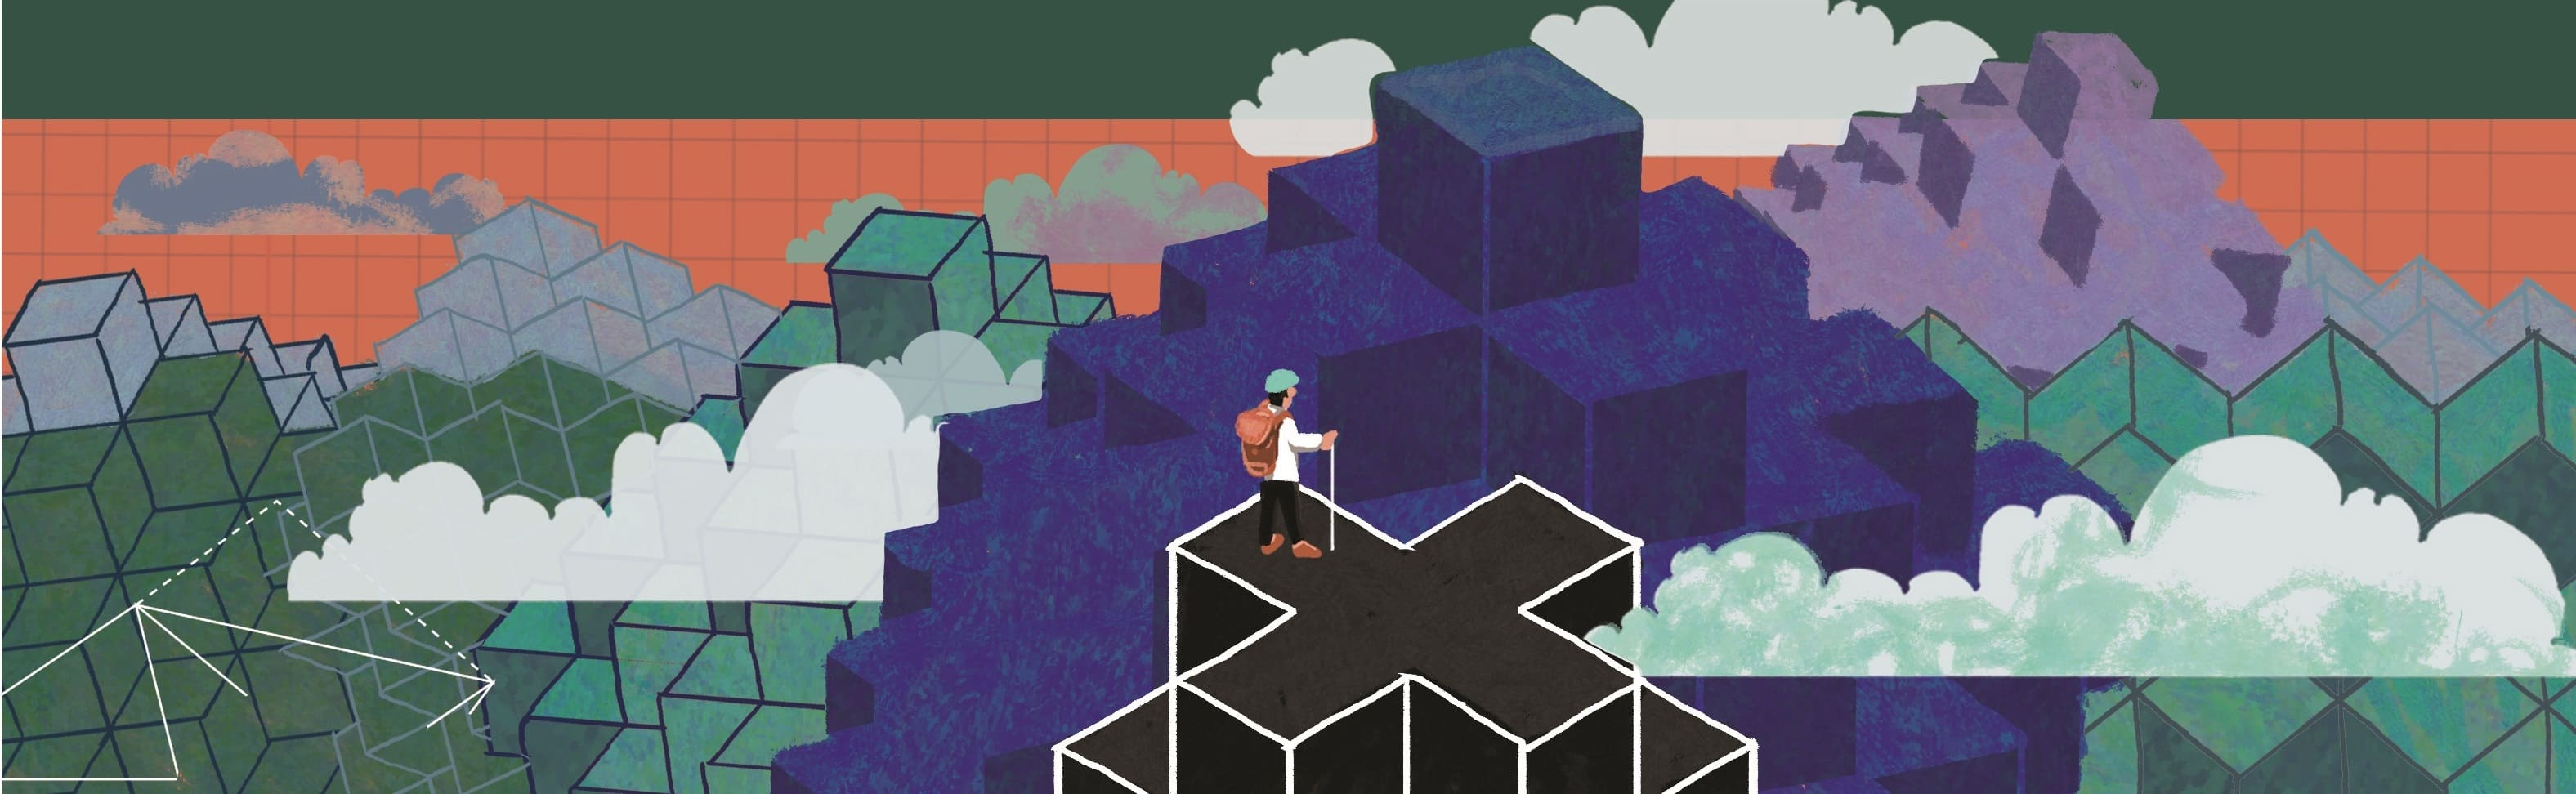
\includegraphics[width=19.3cm]{../thachthuctoanhoc/bannerthachthuc}}}
\centering
\vspace*{4cm}
\endgroup
\vspace*{-8pt}
\begin{tBox}
	\begin{itemize}[leftmargin = 13pt, itemsep = 1.0pt] 
		%		\item Mỗi bài toán đề xuất (kèm theo lời giải) cần được nêu rõ là bài sáng tác hay bài sưu tầm.
		\item Mỗi bài toán đề xuất (kèm theo lời giải) cần được nêu rõ là bài sáng tác hay bài sưu tầm (nếu là bài sưu tầm, cần ghi rõ nguồn).
		\item Bài giải cho mỗi bài toán cần được trình bày trong một file riêng hoặc
		một tờ giấy riêng.
		\item  Người đề xuất bài toán hoặc gửi bài giải cho các bài toán trong mục ``Thách thức kỳ này" cần ghi rõ họ, đệm, tên và nơi làm việc/học tập, số điện thoại liên hệ. Nếu là học sinh (hoặc sinh viên) cần ghi rõ là học sinh lớp mấy (hoặc sinh viên năm thứ mấy).
		\item Các bài toán trong mục Thách thức kỳ này hướng tới các độc giả là học sinh phổ thông; được phân chia thành các mức độ $B$, $A$, và được sắp xếp theo độ khó tăng dần, theo đánh giá chủ quan của Ban biên tập. Các bài toán mức độ $B$ không đòi hỏi các kiến thức vượt quá chương trình môn Toán cấp THCS; các bài toán mức độ $A$ không đòi hỏi các kiến thức vượt quá chương trình môn Toán cấp THPT.
		\item Cách thức gửi bài toán đề xuất hoặc lời giải: gửi file thu được bằng cách scan, ảnh chụp (rõ nét) của bản viết tay, hoặc được soạn thảo bằng các phần mềm Latex, Word tới \url{bbt@pi.edu.vn} hoặc gửi qua đường bưu điện tới Tòa soạn (xem địa chỉ tại bìa $2$).
		\item Hạn gửi lời giải cho các bài toán P$621$--P$630$: trước ngày $15/9/2022$.
	\end{itemize}
\end{tBox}
\begin{center}
	\vspace*{-5pt}
	\textbf{\color{thachthuctoanhoc}THÁCH THỨC KỲ NÀY}
	\vspace*{-5pt}
\end{center}
\begin{multicols}{2}
	\setlength{\abovedisplayskip}{4pt}
	\setlength{\belowdisplayskip}{4pt}
	{\color{thachthuctoanhoc}{\usefont{T5}{qag}{b}{n} P621.}}
	(Mức $B$) Xét ba số nguyên tố có tổng bằng $242$. Hỏi,  tích của chúng lớn nhất bằng bao nhiêu?
	\begin{flushright}
		\textit{Duy Minh, Hà Nội}
	\end{flushright}
	{\color{thachthuctoanhoc}{\usefont{T5}{qag}{b}{n} P622.}}
	(Mức $B$) Cho $x,y,z$ là các số thực khác $0$, thoả mãn 
	\begin{align*}
		\dfrac{x^2+y}{y^2}=\dfrac{y^2+z}{z^2}=\dfrac{z^2+x}{x^2}=2.
	\end{align*}
	Chứng minh rằng $\dfrac x{y^2}+\dfrac y{z^2}+\dfrac z{x^2}$ là một số nguyên.
	\begin{flushright}
		\textit{Trần Quốc Luật, Tp. Hồ Chí Minh}
	\end{flushright}
	{\color{thachthuctoanhoc}{\usefont{T5}{qag}{b}{n} P623.}}
	(Mức $B$) Cho bảng ô vuông kích thước $2023 \times 2023$, mà ở mỗi ô vuông con của nó có ghi một số $1$. Cho phép thay đổi các số trong bảng, theo quy tắc: Mỗi lần, chọn ba ô vuông con tùy ý nằm trong cùng một hàng, hoặc một cột, rồi tăng số đang có ở mỗi ô, trong ba ô đó, lên $1$.
	\vskip 0.05cm
	Hỏi, sau một số hữu hạn lần thực hiện liên tiếp phép thay đổi số nói trên đối với bảng đã cho, ta có thể nhận được bảng $2023 \times 2023$, mà số ở mỗi ô vuông con của nó đều là số chẵn hay không? Vì sao?
	\begin{flushright}
		\textit{Tường Thanh, Nghệ An (st)}
	\end{flushright}
	{\color{thachthuctoanhoc}{\usefont{T5}{qag}{b}{n} P624.}}
	(Mức $B$) Cho tam giác nhọn $ABC$, nội tiếp đường tròn $(O)$. Các đường cao xuất phát từ các đỉnh $B,C$ của tam giác, tương ứng, cắt $(O)$ tại các điểm thứ hai $P,Q$. Gọi $M$ là trung điểm của cạnh $BC$, và gọi $K, L$ tương ứng là hình chiếu vuông góc của $M$ trên $AC, A B$. Các đường thẳng $Q L, P K$ cắt đường thẳng $B C$ tương ứng tại $R, S$. Chứng minh rằng, bốn điểm $P, Q, R, S$ cùng nằm trên một đường tròn.
	\begin{figure}[H]
		\vspace*{-5pt}
		\centering
		\captionsetup{labelformat= empty, justification=centering}
		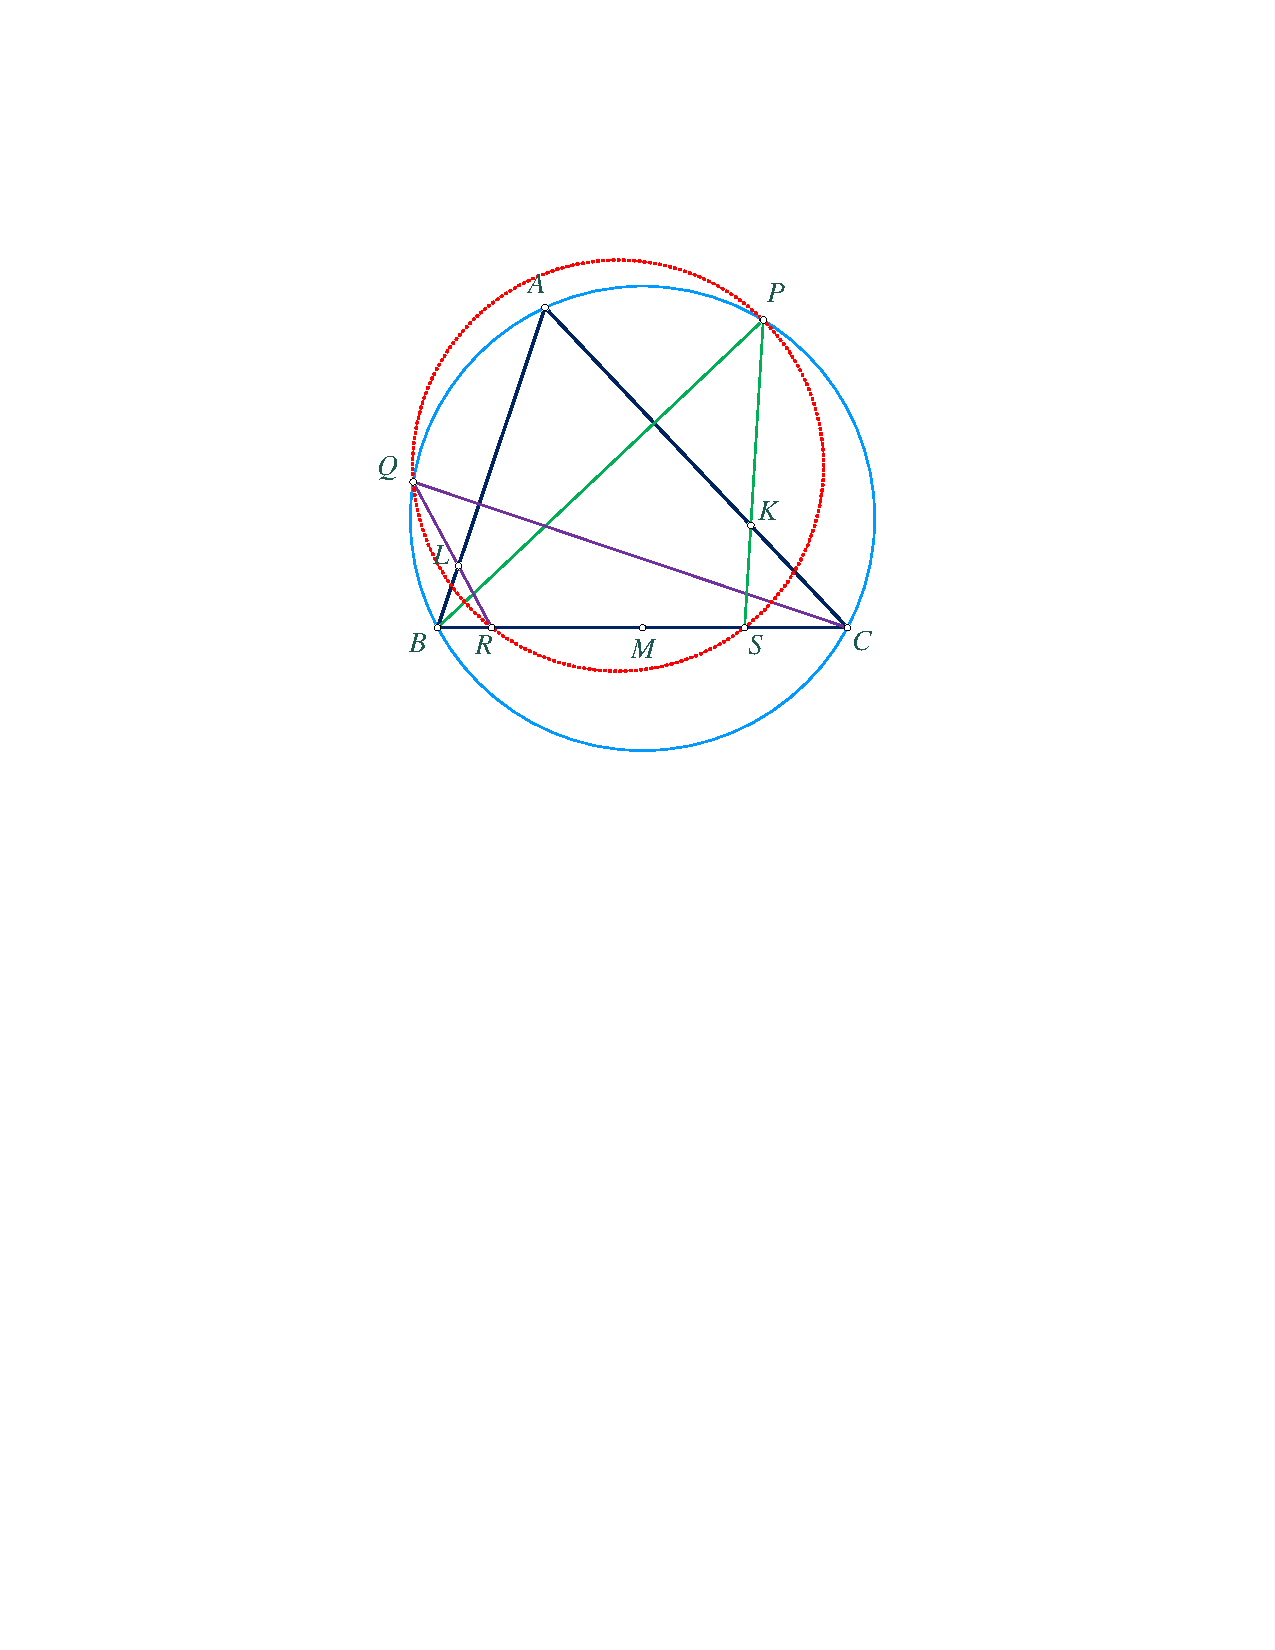
\includegraphics[width= 0.95\linewidth]{P624}
		\vspace*{-15pt}
	\end{figure}
	\begin{flushright}
		\textit{Nguyễn Tiến Dũng, Hà Nội}
	\end{flushright}
	{\color{thachthuctoanhoc}{\usefont{T5}{qag}{b}{n} P625.}}
	(Mức $B$) Cho các số thực dương $a,b,c$. Chứng minh rằng
	\begin{align*}
		\left(\dfrac b{a+c}\right)^2+\left(\dfrac{c}{a+b}\right)^2\ge \dfrac{b^2-bc+c^2}{a^2+bc}.
	\end{align*}
	\begin{flushright}
		\textit{Nguyễn Việt Hùng, Hà Nội}
	\end{flushright}
	{\color{thachthuctoanhoc}{\usefont{T5}{qag}{b}{n} P626.}}
	(Mức $B$) Hỏi, có bao nhiêu tam giác vuông, mà mỗi tam giác có độ dài các cạnh là các số nguyên dương và một trong các cạnh góc vuông có độ dài là $2021^{22}$.
	\begin{flushright}
		\textit{Phạm Nhật Nguyệt, Hải Phòng (st)}
	\end{flushright}
	{\color{thachthuctoanhoc}{\usefont{T5}{qag}{b}{n} P627.}}
	(Mức $A$) Xét $x,y$ là hai số thực dương thoả mãn $xy\ge 1$. Tìm giá trị lớn nhất của biểu thức
	\begin{align*}
		P=\dfrac1{\sqrt{x^2+1}}+\dfrac1{\sqrt{y^2+1}}-\dfrac3{4(x+y)}.
	\end{align*}
	\begin{flushright}
		\textit{Đỗ Xuân Trọng, Hà Nội}
	\end{flushright}
	{\color{thachthuctoanhoc}{\usefont{T5}{qag}{b}{n} P628.}}
	(Mức $A$) Cho tam giác không cân $ABC$ ngoại tiếp đường tròn $(I)$. Gọi $A_1$, $B_1$, $C_1$ tương ứng là tiếp điểm của $BC$, $CA$, $AB$ với $(I)$; $A_2$, $B_2$, $C_2$ lần lượt là điểm đối xứng của $A_1$, $B_1$, $C_1$ tương ứng qua các đường thẳng $B_1C_1$, $C_1A_1$ và $A_1B_1$. Các đường thẳng $AA_2$, $BC$ cắt nhau tại $A_3$; $BB_2$ và $CA$ cắt nhau tại $B_3$; $CC_2$ và $AB$ cắt nhau tại $C_3$. Chứng minh rằng, $A_3$, $B_3$, $C_3$ thẳng hàng.
	\begin{figure}[H]
		\vspace*{-5pt}
		\centering
		\captionsetup{labelformat= empty, justification=centering}
		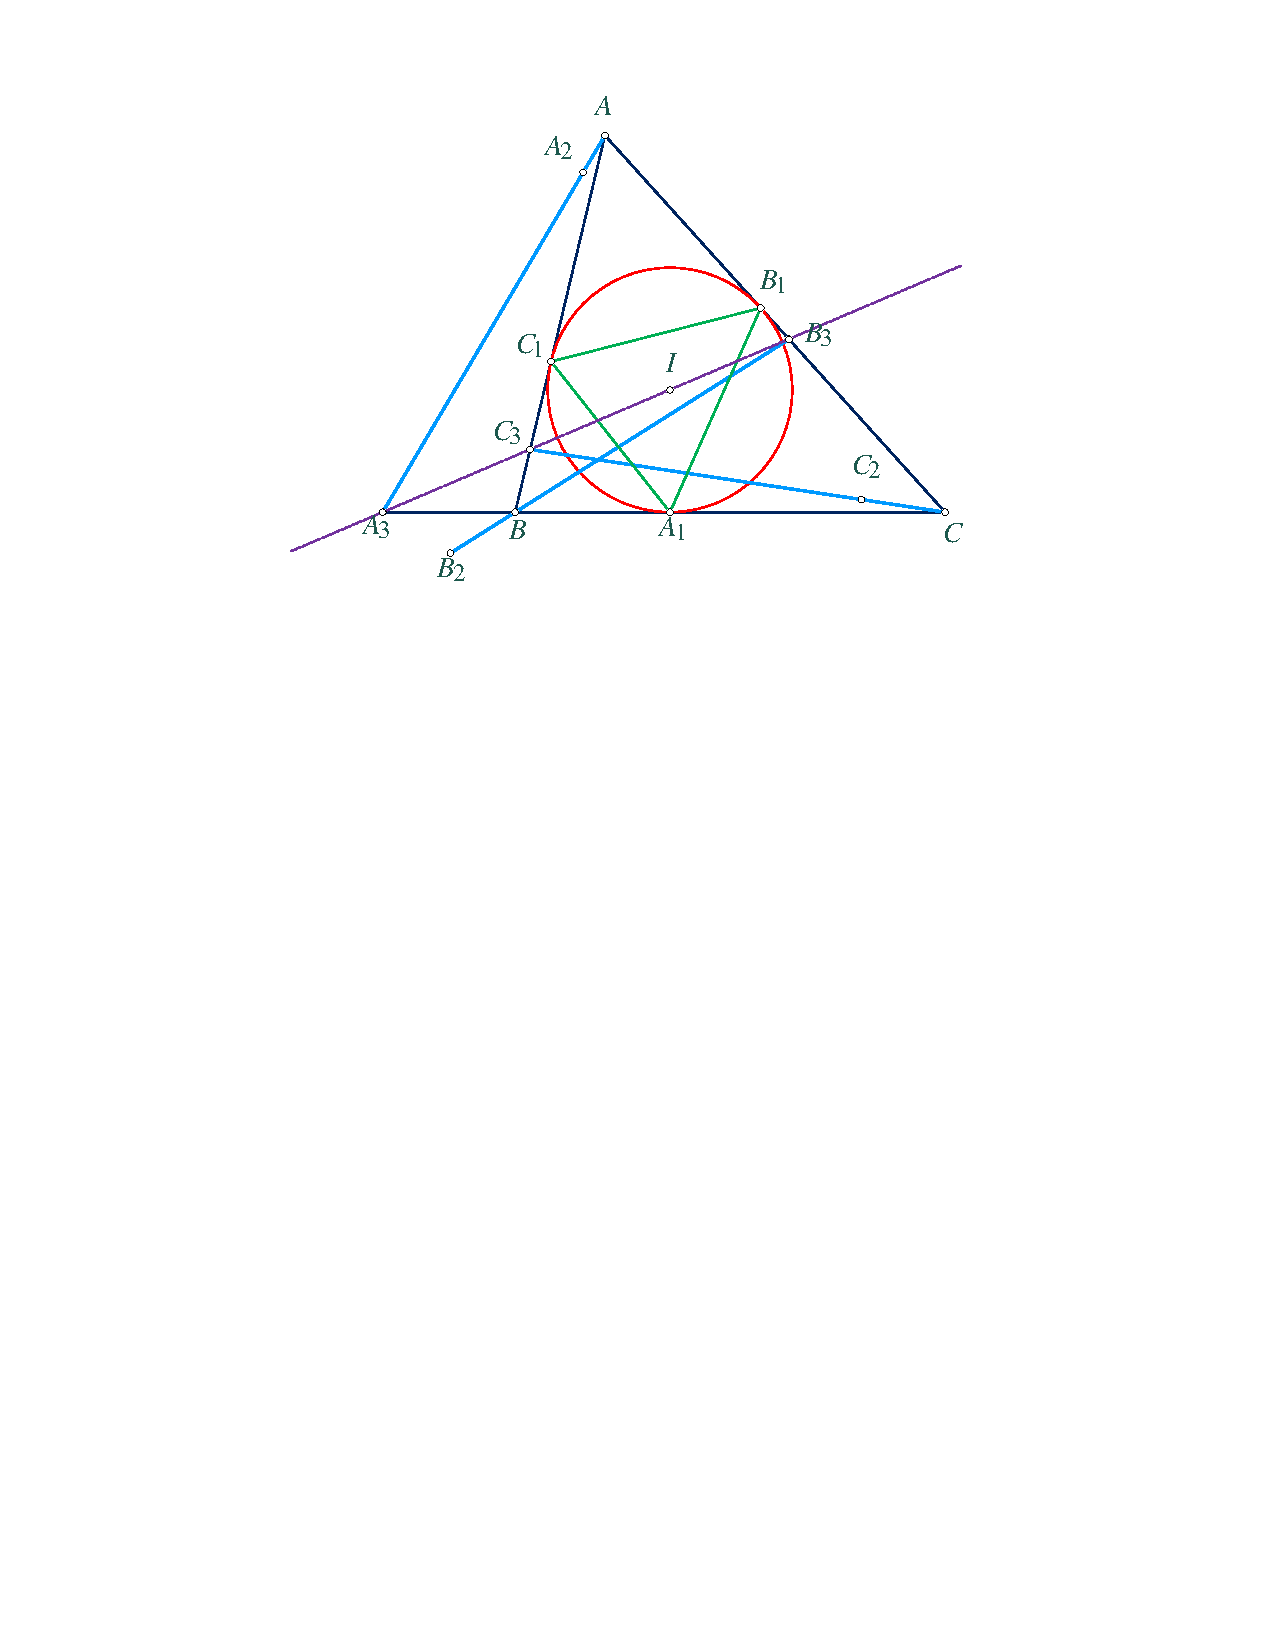
\includegraphics[width= 1.05\linewidth]{P628}
		\vspace*{-15pt}
	\end{figure}
	\begin{flushright}
		\textit{Đậu Anh Hùng, Quảng Trị}
	\end{flushright}
	{\color{thachthuctoanhoc}{\usefont{T5}{qag}{b}{n} P629.}}
	(Mức $A$) Cho $n$ là một số nguyên dương có tính chất: không tồn tại các số nguyên dương $a,b,c$ sao cho 
	\begin{align*}
		\dfrac4n=\dfrac 1a+\dfrac 1b+\dfrac 1c.
	\end{align*}
	Chứng minh rằng, tồn tại các số nguyên không âm $u,v$ sao cho $n=u^2+v^2$.  
	\begin{flushright}
		\textit{Phạm Công Tài, Hà Nội}
	\end{flushright}
	{\color{thachthuctoanhoc}{\usefont{T5}{qag}{b}{n} P630.}}
	(Mức $A$) Bạn Pi ghi lên bảng một số $1$; sau đó, thực hiện việc xoá và ghi thêm số, theo quy tắc:  Mỗi lần, xoá một số $N$ tuỳ ý đang có trên bảng, rồi ghi thêm lên bảng số $N+1$,  hoặc số $3N$.
	\vskip 0.05cm
	Pi thực hiện việc xoá và ghi thêm số, để trên bảng có một số chia hết cho $47$, và Pi dừng việc xoá--ghi thêm số ngay sau khi ghi được một số như vậy. 
	\vskip 0.05cm
	Mỗi lần xoá số $N$ và ghi số $3N$, Pi được nhận một viên kẹo xốp, còn nếu ghi số $N+1$ thì được nhận một viên kẹo dẻo. Vì không thích kẹo dẻo, nên trong quá trình xoá-ghi thêm số, Pi luôn cố gắng để được nhận kẹo xốp. Hỏi, Pi phải nhận ít nhất bao nhiêu viên kẹo dẻo? 
	\begin{flushright}
		\textit{Trần Nguyễn Nam Hưng, Tp. Hồ Chí Minh}
	\end{flushright}
\end{multicols}
\begin{center}
	{\large{\textbf{\color{thachthuctoanhoc}GIẢI BÀI KỲ TRƯỚC}}}
\end{center}
\begin{multicols}{2}
	\setlength{\abovedisplayskip}{4pt}
	\setlength{\belowdisplayskip}{4pt}
	{\color{thachthuctoanhoc}{\usefont{T5}{qag}{b}{n} P591.}}
	(Mức $B$) Xét bốn số thực phân biệt có tính chất: mỗi số $189$, $264$, $287$, $320$ đều là tổng của hai trong bốn số ấy. Hỏi, tổng của bốn số đó có thể lớn nhất là bao nhiêu?
	\vskip 0.05cm
	\textbf{\color{thachthuctoanhoc}Lời giải} \textit{(phỏng theo ý giải của bạn Trần Minh Hoàng, lớp $9$E, trường THCS Nguyễn Trãi, huyện Nghi Xuân, tỉnh Hà Tĩnh})\textbf{\color{thachthuctoanhoc}.}
	\vskip 0.05cm
	Gọi $a$, $b$, $c$, $d$ là bốn số thực có tính chất đã nêu trong đề bài.
	\vskip 0.05cm
	Khi đó, $189$, $264$, $287$, $320$ là bốn trong sáu số: $a + b$, $c + d$, $a + c$, $b + d$, $a + d$, $b + c$. Do đó, bốn số vừa nêu thuộc ba nhóm số $\{a \!+\! b; c \!+\! d\}$, $\{a \!+\! c; b \!+\! d\}$ và $\{a \!+\! d; b \!+\! c\}$. Suy ra, phải có hai trong bốn số ấy thuộc cùng một nhóm. Do hai số đó là hai số phân biệt nên tổng của chúng chính là tổng của hai số trong nhóm. Từ đây, vì tổng của hai số cùng nhóm nào cũng bằng $a + b + c + d$, nên suy ra trong bốn số $189$, $264$, $287$, $320$ phải có hai số có tổng bằng $a + b + c + d$. Vì thế, ta có:
	\begin{align*}
		a + b + c + d &\le 287 + 320\\
		 &= 607.
	\end{align*}
	Hơn nữa, nhận thấy, bốn số $83$, $106$, $181$, $237$ có tính chất đã nêu trong đề bài (vì $189 = 83 + 106$, $264 = 83 + 181$,\linebreak $287 = 106 + 181$, $320 = 83 + 237$) và tổng của chúng bằng
	\begin{align*}
		83 + 106 + 181 + 237 = 607.
	\end{align*}
	Vì vậy, tổng của bốn số có tính chất đã nêu trong đề bài có thể lớn nhất bằng $607$.
	\vskip 0.05cm
	\textbf{\color{thachthuctoanhoc}Bình luận và Nhận xét}
	\vskip 0.05cm
	Ngoài lời giải của bạn \textit{Trần Minh Hoàng}, Tạp chí đã nhận được hai lời giải nữa; trong đó, có một lời giải sai, và một lời giải không hoàn chỉnh, vì mắc lỗi logic (cụ thể, người giải bài đã khẳng định giá trị lớn nhất của tổng $a + b + c + d$ bằng $607$, ngay sau khi mới chỉ chứng minh được tổng đó không vượt quá $607$).
	\vskip 0.05cm
	\hfill	\textbf{\color{thachthuctoanhoc}Lê Huy}
	\vskip 0.05cm
	{\color{thachthuctoanhoc}{\usefont{T5}{qag}{b}{n} P592.}}
	(Mức $B$) Tìm chữ số hàng đơn vị của số 
	\begin{align*}
		A=&\left(1+2^2+3^3+\cdots+2022^{2022}\right)\\
		&\cdot\left(5^5+15^{15}+25^{25}+\cdots +2025^{2025}\right).
	\end{align*}
	\textbf{\color{thachthuctoanhoc}Lời giải} (\textit{dựa theo lời giải của bạn Hà Mạnh Hùng, lớp $7$A, trường THPT chuyên Hà Nội -- Amsterdam, Tp. Hà Nội})\textbf{\color{thachthuctoanhoc}.}
	\vskip 0.05cm
	Đặt  $B = 1 + {2^2} + {3^3} +  \cdots  + {2022^{2022}}$ và $C = {5^5} + {15^{15}} + {25^{25}} +  \cdots  + {2025^{2025}}$.
	\vskip 0.05cm 
	Ta có:
	\begin{align*}
		B = &\left( {1 + {2^2}} \right) + \left( {{3^3} + {4^4}} \right) +  \cdots\\
		  &+ \left( {{{2021}^{2021}} + {{2022}^{2022}}} \right).
	\end{align*}
	Dễ thấy, tổng của hai số trong mỗi ``ngoặc đơn" là một số lẻ, và có tất cả $2022 : 2 = 1011$ ``ngoặc đơn". Do đó, $B$ là tổng của một số lẻ các số lẻ. Vì thế, $B$ là một số lẻ.   \hfill ($1$)
	\vskip 0.05cm
	Tiếp theo, nhận thấy, mỗi số hạng của tổng $C$ là một số lẻ chia hết cho $5$, và tổng đó có $(2025 - 5) : 10 + 1 = 203$ số hạng. Do đó, $C$ là tổng của một số lẻ các số lẻ chia hết cho $5$. Vì thế, $C$ là một số lẻ, chia hết cho $5$. \hfill ($2$)
	\vskip 0.05cm
	Từ ($1$) và ($2$) suy ra, $A = B \cdot C$  là một số lẻ, chia hết cho $5$. Vì thế, chữ số tận cùng, hay chữ số hàng đơn vị, của $A$ là $5$.
	\vskip 0.05cm
	\textbf{\color{thachthuctoanhoc}Bình luận và Nhận xét}
	\vskip 0.05cm
	Tất cả các lời giải Tạp chí nhận được từ bạn đọc đều có ý giải đúng. Tuy nhiên, một số lời giải trong số đó không hoàn chỉnh do người giải bài đã tính sai số số hạng của tổng $C$ (trong lời giải trên), hoặc lời giải được trình bày quá vắn tắt, thiếu các lý giải cần thiết.
	\vskip 0.05cm
	\hfill	\textbf{\color{thachthuctoanhoc}Lưu Thị Thanh Hà}
	\vskip 0.05cm
	{\color{thachthuctoanhoc}{\usefont{T5}{qag}{b}{n} P593.}}
	(Mức $B$) Cho $n$ là một số nguyên dương. Chứng minh rằng, nếu $4n+1$ và $20n+1$ là các số chính phương thì $20n+21$ là một hợp số.
	\vskip 0.05cm
	\textbf{\color{thachthuctoanhoc}Lời giải} (\textit{dựa theo lời giải của bạn Trần Minh Hoàng, lớp $9$E, trường THCS Nguyễn Trãi, huyện Nghi Xuân, tỉnh Hà Tĩnh})\textbf{\color{thachthuctoanhoc}.}
	\vskip 0.05cm
	Ta biết rằng, khi chia một số chính phương cho $3$ sẽ được số dư là $0$ hoặc $1$. Vì thế, từ giả thiết $4n + 1$ và $20n + 1$ là các số chính phương, suy ra, hoặc $4n + 1$ và $20n + 1$ cùng chia hết cho $3$ (tức, chia $3$ dư $0$), hoặc trong hai số $4n + 1$ và $20n + 1$ có ít nhất một số chia $3$ dư $1$.
	\vskip 0.05cm
	Nếu $4n + 1$ và $20n + 1$ cùng chia hết cho $3$ thì
	\begin{align*}
		(20n + 1) - (4n + 1) = 16n
	\end{align*}
	chia hết cho $3$. Suy ra, $n$ chia hết cho $3$ (do $16$ và $3$ nguyên tố cùng nhau). Vì thế, $4n$ và $20n$ chia hết cho $3$; suy ra, $1$ chia hết cho $3$, là điều vô lý. Vì vậy, phải có: trong hai số $4n + 1$ và $20n + 1$ có ít nhất một số chia $3$ dư $1$. Khi đó, trong hai số $4n$ và $20n$ có ít nhất một số chia hết cho $3$. Từ đây, vì $4$ và $3$ nguyên tố cùng nhau, $20$ và $3$ nguyên tố cùng nhau, suy ra, $n$ chia hết cho $3$. Vì thế, $20n + 21$ chia hết cho $3$. Mà $20n + 21 > 3$, nên $20n + 21$ là hợp~số.
	\vskip 0.05cm
	Ta có điều phải chứng minh theo yêu cầu đề bài.
	\vskip 0.05cm
	\textbf{\color{thachthuctoanhoc}Bình luận và Nhận xét}
	\vskip 0.05cm
	Rất tiếc, trong số các lời giải Tạp chí đã nhận được từ bạn đọc, có một lời giải sai, do người giải bài đã mắc \textbf{\color{thachthuctoanhoc}\textit{lỗi}} sau: ``Với $a$, $b$, $c$ là các số nguyên dương, từ  $a = b \cdot c$ và $b > 1$, suy ra, $a$ là hợp số.". (\textit{Khẳng định vừa nêu hiển nhiên sai, nếu $c = 1$ và $b$ là số nguyên tố.}). Ngoài lời giải sai vừa nêu, tất cả các lời giải còn lại đều là lời giải đúng và hoàn chỉnh.
	\vskip 0.05cm
	\hfill	\textbf{\color{thachthuctoanhoc}Lưu Thị Thanh Hà}
	\vskip 0.05cm
	{\color{thachthuctoanhoc}{\usefont{T5}{qag}{b}{n} P594.}}
	(Mức $B$) Giải phương trình:
	\begin{align*}
		&\sqrt{1+2 x}+\sqrt{1-2 x}\\
		=&(1+3 x) \sqrt{1-3 x}+(1-3 x) \sqrt{1+3 x}.
	\end{align*}
	\textbf{\color{thachthuctoanhoc}Lời giải} (\textit{dựa theo cách giải của bạn Nguyễn Đức Khải, lớp $10$T$2$, trường THPT chuyên Lê Hồng Phong, tỉnh Nam Định}).
	\vskip 0.05cm
	Điều kiện xác định của phương trình:
	\begin{align*}
		-\dfrac{1}{3} \le x \le \dfrac{1}{3}.
	\end{align*}
	Với điều kiện đó, phương trình đã cho tương đương với phương trình
	\begin{align*}
		&\sqrt {1 + 2x}  + \sqrt {1 - 2x}  \\
		= &\sqrt {1 - 9{x^2}} \left( {\sqrt {1 + 3x}  + \sqrt {1 - 3x} } \right).
	\end{align*}
	Vì thế, giả sử $x_0$  là nghiệm của phương trình đã cho, ta có $ - \dfrac{1}{3} \le {x_0} \le \dfrac{1}{3}$  và
	\begin{align*}
		&\sqrt {1 + 2{x_0}}  + \sqrt {1 - 2{x_0}}  \\
		= &\sqrt {\!1 \!-\! 9x_0^2} \left(\!\sqrt {1 \!+\! 3{x_0}}  \!+\! \sqrt {1 \!-\! 3{x_0}}  \right). \tag{$1$}
	\end{align*}
	Ký hiệu $VP$ là vế phải của ($1$).\\
	Do $0 \le \sqrt {1 - 9x_0^2}  \le 1$  nên
	\begin{align*}
		VP \le \sqrt {1 + 3{x_0}}  + \sqrt {1 - 3{x_0}} .
	\end{align*}
	Do đó, từ ($1$) suy ra
	\begin{align*}
		&\sqrt {1 + 2{x_0}}  + \sqrt {1 - 2{x_0}}  \\
		\le &\sqrt {1 + 3{x_0}}  + \sqrt {1 - 3{x_0}}. \tag{$2$}
	\end{align*}
	Ta có:
	\begin{align*}
		(2) &\Leftrightarrow 2 + 2\sqrt {1 - 4x_0^2}  \le 2 + 2\sqrt {1 - 9x_0^2} \\
		&\Leftrightarrow \sqrt {1 - 4x_0^2}  \le \sqrt {1 - 9x_0^2} \\
		&\Leftrightarrow 1 - 4x_0^2 \le 1 - 9x_0^2 \Leftrightarrow x_0^2 \le 0.
	\end{align*}  
	Vì thế,  $x_0 = 0$.
	\vskip 0.05cm
	Ngược lại, bằng cách thử trực tiếp, ta thấy, $x = 0$ nghiệm đúng phương trình đã cho.
	\vskip 0.05cm
	Vậy, phương trình đã cho có duy nhất nghiệm $x = 0$.
	\vskip 0.05cm
	\textbf{\color{thachthuctoanhoc}Bình luận và Nhận xét}
	\vskip 0.05cm
	$\pmb{1.}$ Hầu hết các lời giải Tạp chí đã nhận được từ bạn đọc đều là lời giải theo cách sử dụng phép bình phương hai vế của phương trình để thực hiện các biến đổi tương đương. Lời giải theo cách này khá dài dòng và cồng kềnh.
	\vskip 0.05cm
	$\pmb{2.}$ Tất cả các lời giải Tạp chí nhận được từ bạn đọc đều là lời giải đúng và hoàn chỉnh.
	\vskip 0.05cm
	\hfill	\textbf{\color{thachthuctoanhoc}Lê Huy}
	\vskip 0.05cm
	{\color{thachthuctoanhoc}{\usefont{T5}{qag}{b}{n} P595.}}
	(Mức $B$) Cho tam giác nhọn, không cân $ABC$ nội tiếp $(O)$, có các đường cao $AD,BE,CF$. Gọi $G$ là giao điểm của các đường thẳng $BC,EF$. Đường tròn ngoại tiếp tam giác  $ADG$ cắt $(O)$ tại điểm thứ hai $I$ (khác  $A$). Các đường thẳng $AI$ và $EF$ cắt nhau tại $K$. Chứng minh rằng, đường thẳng nối $K$ và trực tâm của tam giác $ABC$  đi qua trung điểm của $BC$.
	\begin{figure}[H]
		\vspace*{-5pt}
		\centering
		\captionsetup{labelformat= empty, justification=centering}
		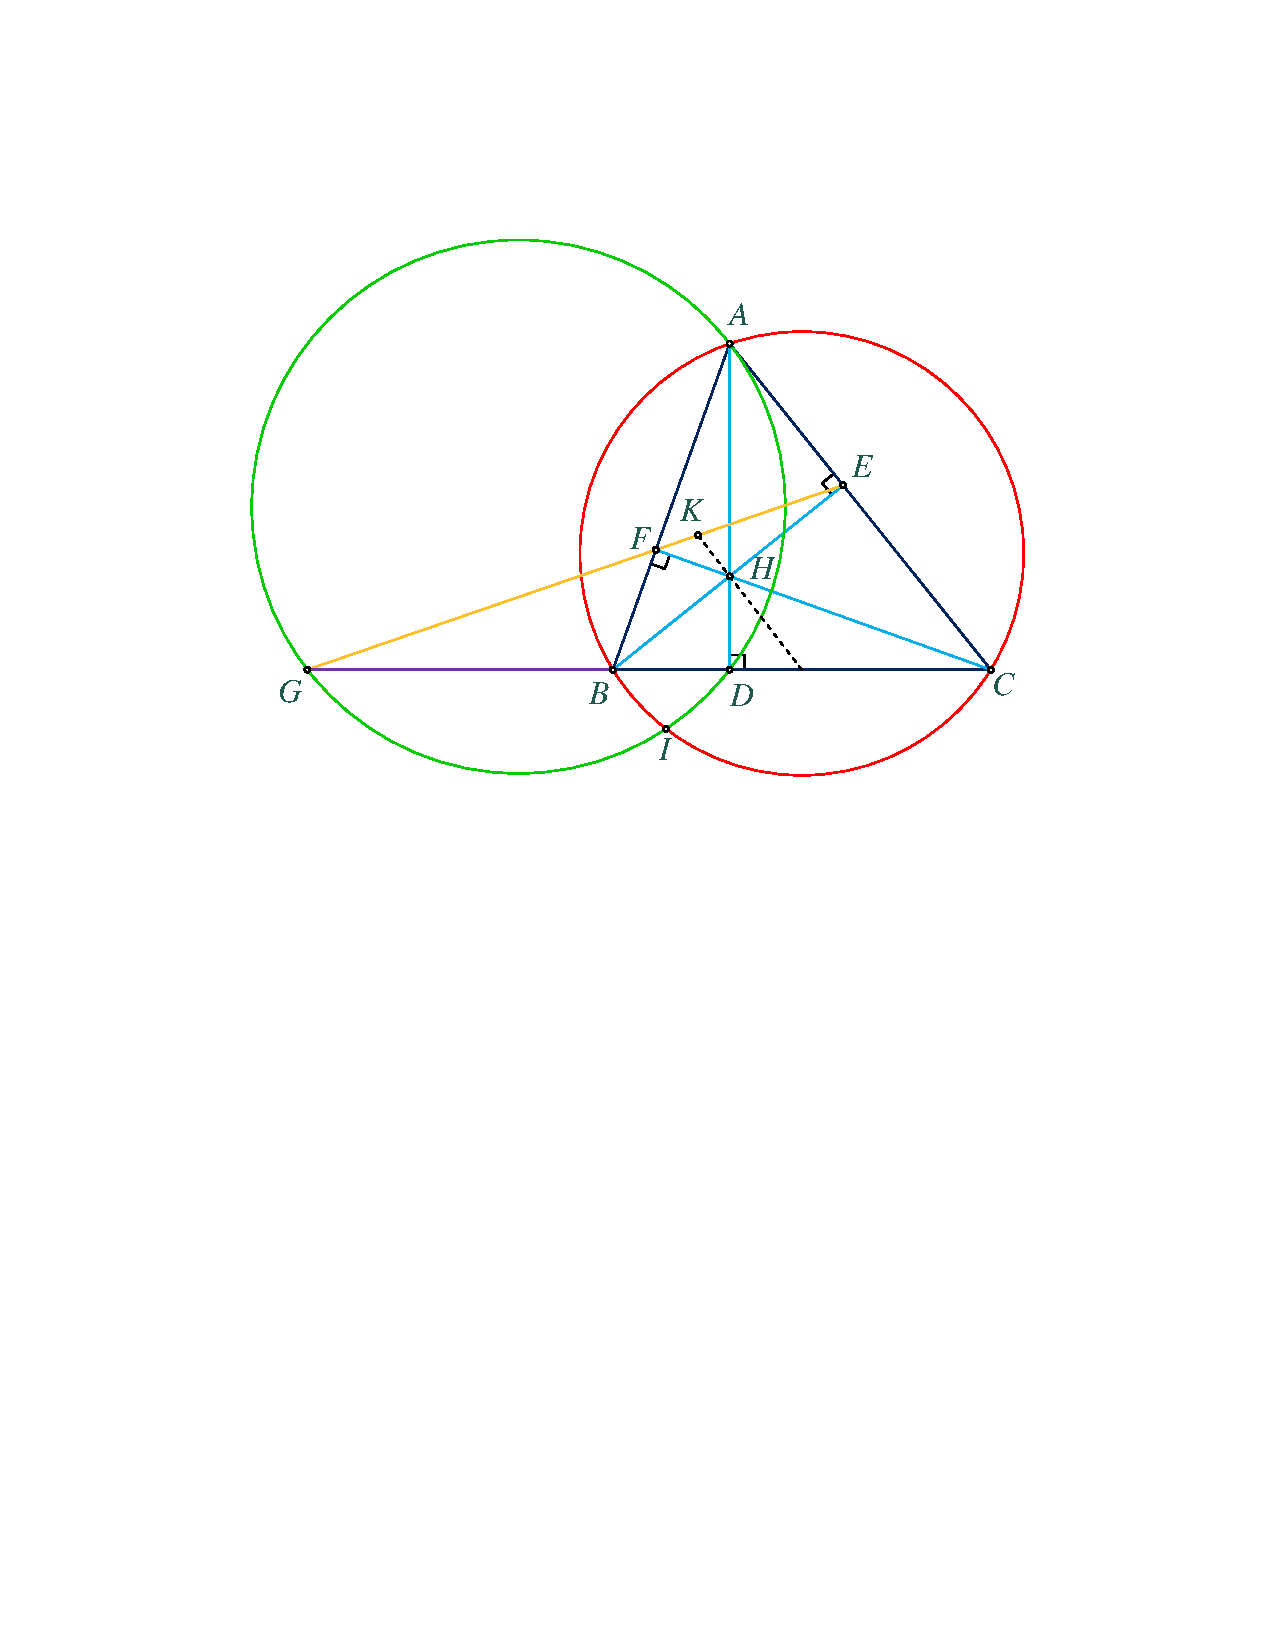
\includegraphics[width= 0.99\linewidth]{P595}
		\vspace*{-10pt}
	\end{figure}
	\textbf{\color{thachthuctoanhoc}Lời giải} (\textit{của người chấm bài})\textbf{\color{thachthuctoanhoc}.}
	\vskip 0.05cm
	Trước hết, ta nhắc lại (không chứng minh) hai kết quả cơ bản sau:
	\vskip 0.05cm
	\textbf{\color{thachthuctoanhoc}Kết quả} $\pmb{1.}$ Cho tam giác $ABC$ nội tiếp đường tròn $(O)$. Gọi $H$ là trực tâm của tam giác đó; gọi $M$ là trung điểm cạnh $BC$; và gọi $N$ là điểm đối xứng với $H$ qua $M$. Khi đó, $AN$ là một đường kính của $(O)$.
	\vskip 0.05cm
	\textbf{\color{thachthuctoanhoc}Kết quả} $\pmb{2.}$ Cho tam giác $ABC$ nội tiếp đường tròn $(O)$. Gọi $E, F$, tương ứng, là chân các đường cao kẻ từ $B, C$ của tam giác đó; ta có $AO \bot EF$.
	\vskip 0.05cm
	\textit{Trở lại bài toán}.
	\begin{figure}[H]
		\vspace*{-5pt}
		\centering
		\captionsetup{labelformat= empty, justification=centering}
		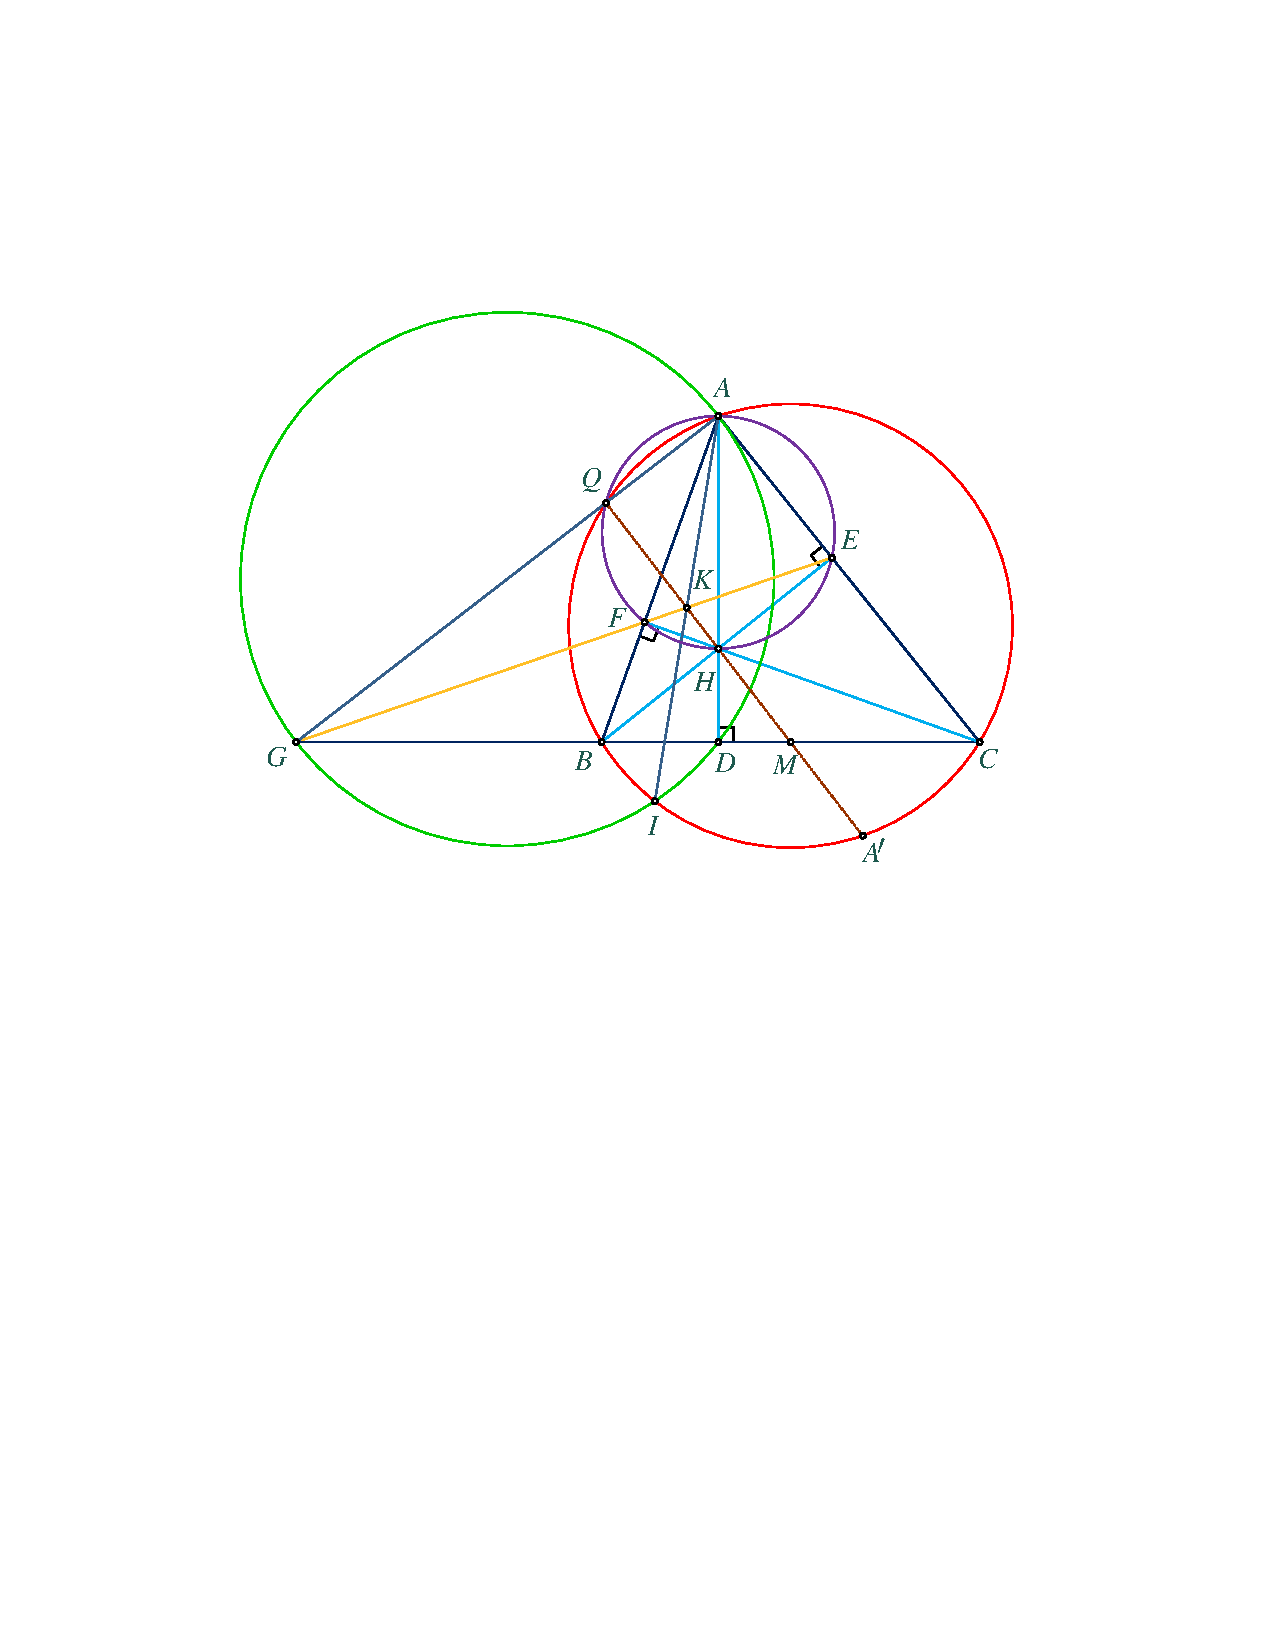
\includegraphics[width= 0.99\linewidth]{P595a}
		\vspace*{-10pt}
	\end{figure}
	Gọi $H$ là trực tâm của tam giác $ABC$; gọi $M$ là trung điểm cạnh $BC$; và gọi $N$ là điểm đối xứng với $H$ qua $M$.
	\vskip 0.05cm
	Theo Kết quả $1$, $AN$ là một đường kính của $(O)$.  \hfill   ($1$)
	\vskip 0.05cm
	Do đó, $\angle AIN = 90^\circ$ \hfill ($2$)
	\vskip 0.05cm
	Từ định nghĩa điểm $D$ suy ra, $AG$ là đường kính của đường tròn $(ADG)$. Vì thế, $\angle AIG = 90^\circ$.  Kết hợp với ($2$), suy ra, ba điểm $G, I, N$ thẳng hàng. Do đó, $AI \bot GN$. \hfill  ($3$)
	\vskip 0.05cm
	Tiếp theo, theo Kết quả $2$, ta có $AN \bot GE$. Từ đây và ($3$) suy ra, $K$ là trực tâm tam giác $AGN$. Do đó, $NK \bot AG$. \hfill ($4$)
	\vskip 0.05cm
	Gọi $L$ là giao điểm thứ hai (khác $A$) của $AG$  và $(O)$. Từ ($1$) suy ra, $\angle ALN = 90^\circ$. \hfill  ($5$)
	\vskip 0.05cm
	Từ định nghĩa của các điểm $H$, $E$, $F$ dễ thấy, $BCEF$ và $HEAF$ là các tứ giác nội tiếp. Xét phương tích của điểm $G$ đối với các đường tròn $(O)$, $(BCEF)$ và $(HEAF)$, ta có:
	\begin{align*}
		GL \cdot GA &= {P_{G/(O)}} = GB \cdot GC = {P_{G/(BCEF)}} \\
		&= GE \cdot GF = {P_{G/(HEAF)}}.
	\end{align*}
	Suy ra, $L$ thuộc đường tròn $(HEAF)$; mà $AH$ là đường kính của đường tròn này, nên $\angle ALH = 90^\circ$. Kết hợp với ($5$), suy ra, ba điểm $N$, $H$, $L$ thẳng hàng; do đó, \linebreak$NH \bot AG$. \hfill ($6$)
	\vskip 0.05cm
	Từ ($4$) và ($6$) suy ra, ba điểm $N$, $H$, $K$ thẳng hàng. Mà $N$, $H$, $M$ là ba điểm thẳng hàng nên $M$, $H$, $K$ là ba điểm thẳng hàng. Ta có điều phải chứng minh theo yêu cầu đề bài.
	\vskip 0.05cm
	\textbf{\color{thachthuctoanhoc}Bình luận và Nhận xét}
	\vskip 0.05cm
	$\pmb{1.}$ Với các giả thiết của bài ra, ta còn có thể chứng minh được: $GH \bot AM$, và đường thẳng $KD$ đi qua giao điểm hai tiếp tuyến tại $B, C$ của $(O)$.
	\vskip 0.05cm
	$\pmb{2.}$ Tất cả các lời giải Tạp chí đã nhận được từ bạn đọc đều là lời giải đúng và hoàn chỉnh.
	\vskip 0.1cm
	\hfill	\textbf{\color{thachthuctoanhoc}Hạ Vũ Anh}
	\vskip 0.1cm
	{\color{thachthuctoanhoc}{\usefont{T5}{qag}{b}{n} P596.}}
	(Mức $B$) Cho các số thực không âm $a,b,c$ thoả mãn $a^2+b^2+c^2=2$. Chứng minh rằng
	\begin{align*}
		8(2\!-\!a\!-\!b)(2\!-\!b\!-\!c)(2\!-\!c\!-\!a)\ge(abc)^2.
	\end{align*}
	Đẳng thức xảy ra khi nào?
	\vskip 0.05cm
	\textbf{\color{thachthuctoanhoc}Lời giải} (\textit{dựa theo cách giải của đa số lời giải Tạp chí đã nhận được từ bạn đọc})\textbf{\color{thachthuctoanhoc}.}
	\vskip 0.05cm
	Từ giả thiết của bài ra, ta có:
	\begin{align*}
		&2\left( {2 - a - b} \right) \\
		= \,&4 - 2a - 2b \\
		= \,&{a^2} + {b^2} + {c^2} - 2a - 2b + 2 \\
		= \,&{\left( {a - 1} \right)^2} + {\left( {b - 1} \right)^2} + {c^2} \ge {c^2}. \tag{$1$}
	\end{align*}
	Bằng cách hoàn toàn tương tự, ta cũng chứng minh được:
	\begin{align*}
		&2\left( {2 - b - c} \right) \ge {a^2}.\tag{$2$}\\
		&2\left( {2 - c - a} \right) \ge {b^2}.\tag{$3$}
	\end{align*}
	Vì các vế của các bất đẳng thức cùng chiều ($1$), ($2$), ($3$) đều là các số không âm (do  $a^2$, $b^2$, $c^2 \ge 0$), nên nhân các bất đẳng thức đó, vế theo vế, ta nhận được bất đẳng thức cần chứng minh theo yêu cầu đề bài.
	\vskip 0.05cm
	Dễ thấy, đẳng thức xảy ra khi và chỉ khi trong ba số $a, b, c$ có hai số bằng $1$ và số còn lại bằng $0$.
	\vskip 0.05cm
	\textbf{\color{thachthuctoanhoc}Bình luận và Nhận xét}
	\vskip 0.05cm
	Rất tiếc, trong số các lời giải Tạp chí đã nhận được từ bạn đọc, có một lời giải không hoàn chỉnh, do người giải bài chưa nêu câu trả lời cho câu hỏi ``Đẳng thức xảy ra khi nào?" của đề bài. Tất cả các lời giải còn lại đều là lời giải hoàn chỉnh.
	\vskip 0.05cm
	\hfill	\textbf{\color{thachthuctoanhoc}Lê Huy}
	\vskip 0.05cm
	{\color{thachthuctoanhoc}{\usefont{T5}{qag}{b}{n} P597.}}
	(Mức $A$) 
	Một nhà địa chất đang ở vị trí $A$ trong sa mạc, cách con đường thẳng $10$ km ($AN = 10$ km). Trên con đường thì xe của nhà địa chất có thể chạy với vận tốc tối đa $50$ km/h nhưng trên sa mạc thì nó chỉ chạy được với vận tốc tối đa $30$ km/h. 
	\begin{figure}[H]
		\centering
		\vspace*{-10pt}
		\captionsetup{labelformat= empty, justification=centering}
		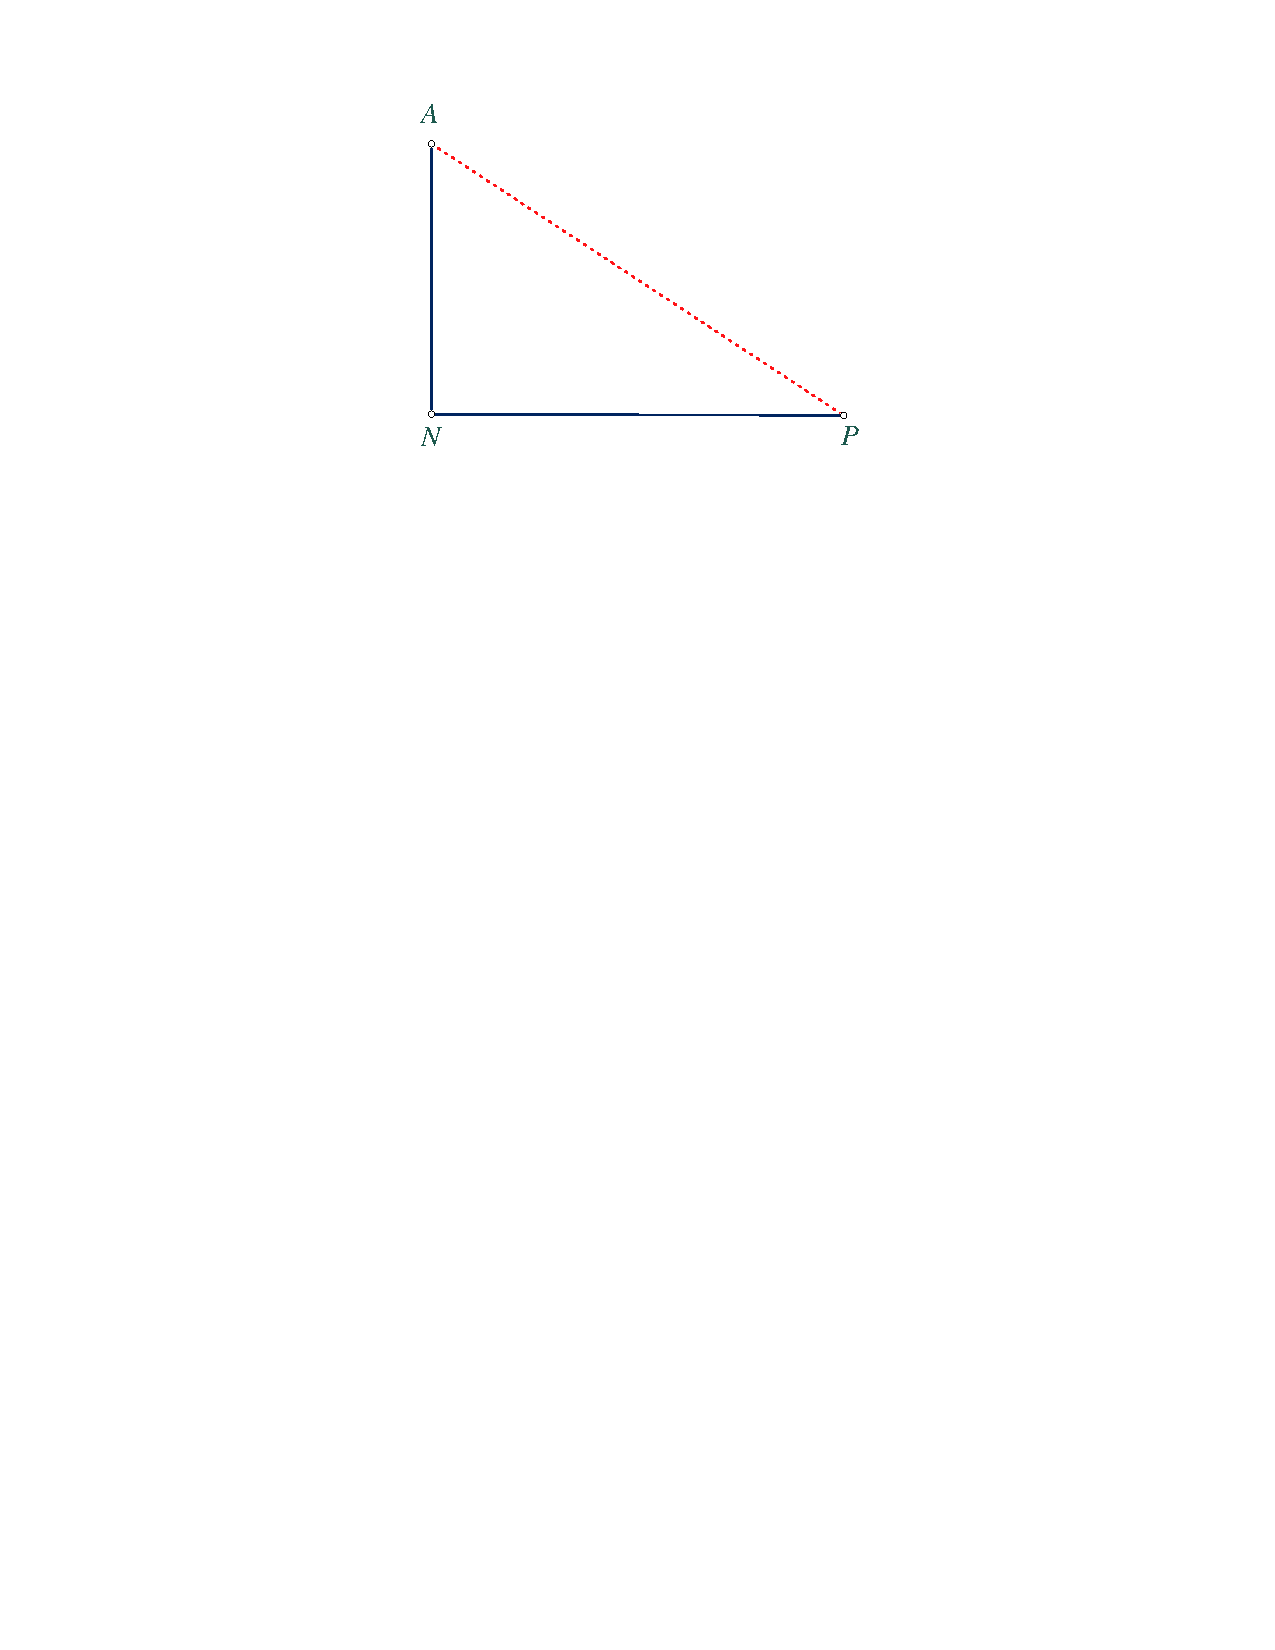
\includegraphics[width=0.8\linewidth]{P597}
		\vspace*{-10pt}
	\end{figure}
	Nhà địa chất đang rất khát nước và ông biết rằng có một trạm xăng $P$ ở vị trí xuôi theo đường $25$ km ($NP = 25$ km) và ở đó có bán nước giải khát.  
	\vskip 0.05cm
	$a)$ Nhà địa chất tốn ít nhất bao nhiêu phút để đi từ $A$ đến $P$ theo đường sa mạc?
	\vskip 0.05cm
	$b)$ Nếu nhà địa chất đi từ $A$ đến $N$, sau đó sử dụng con đường để đến $P$ thì có nhanh hơn không?
	\vskip 0.05cm
	$c)$ Hãy tìm một cách đi nhanh hơn cho nhà địa chất. Cách của bạn đã là nhanh nhất chưa?
	\vskip 0.05cm
	\textbf{\color{thachthuctoanhoc}Lời giải} (\textit{dựa theo lời giải của bạn Võ Khắc Minh Hoàng, lớp $10$ Toán $2$, trường THPT chuyên Quốc học Huế, tỉnh Thừa Thiên -- Huế})\textbf{\color{thachthuctoanhoc}.}
	\begin{figure}[H]
		\centering
		\vspace*{-10pt}
		\captionsetup{labelformat= empty, justification=centering}
		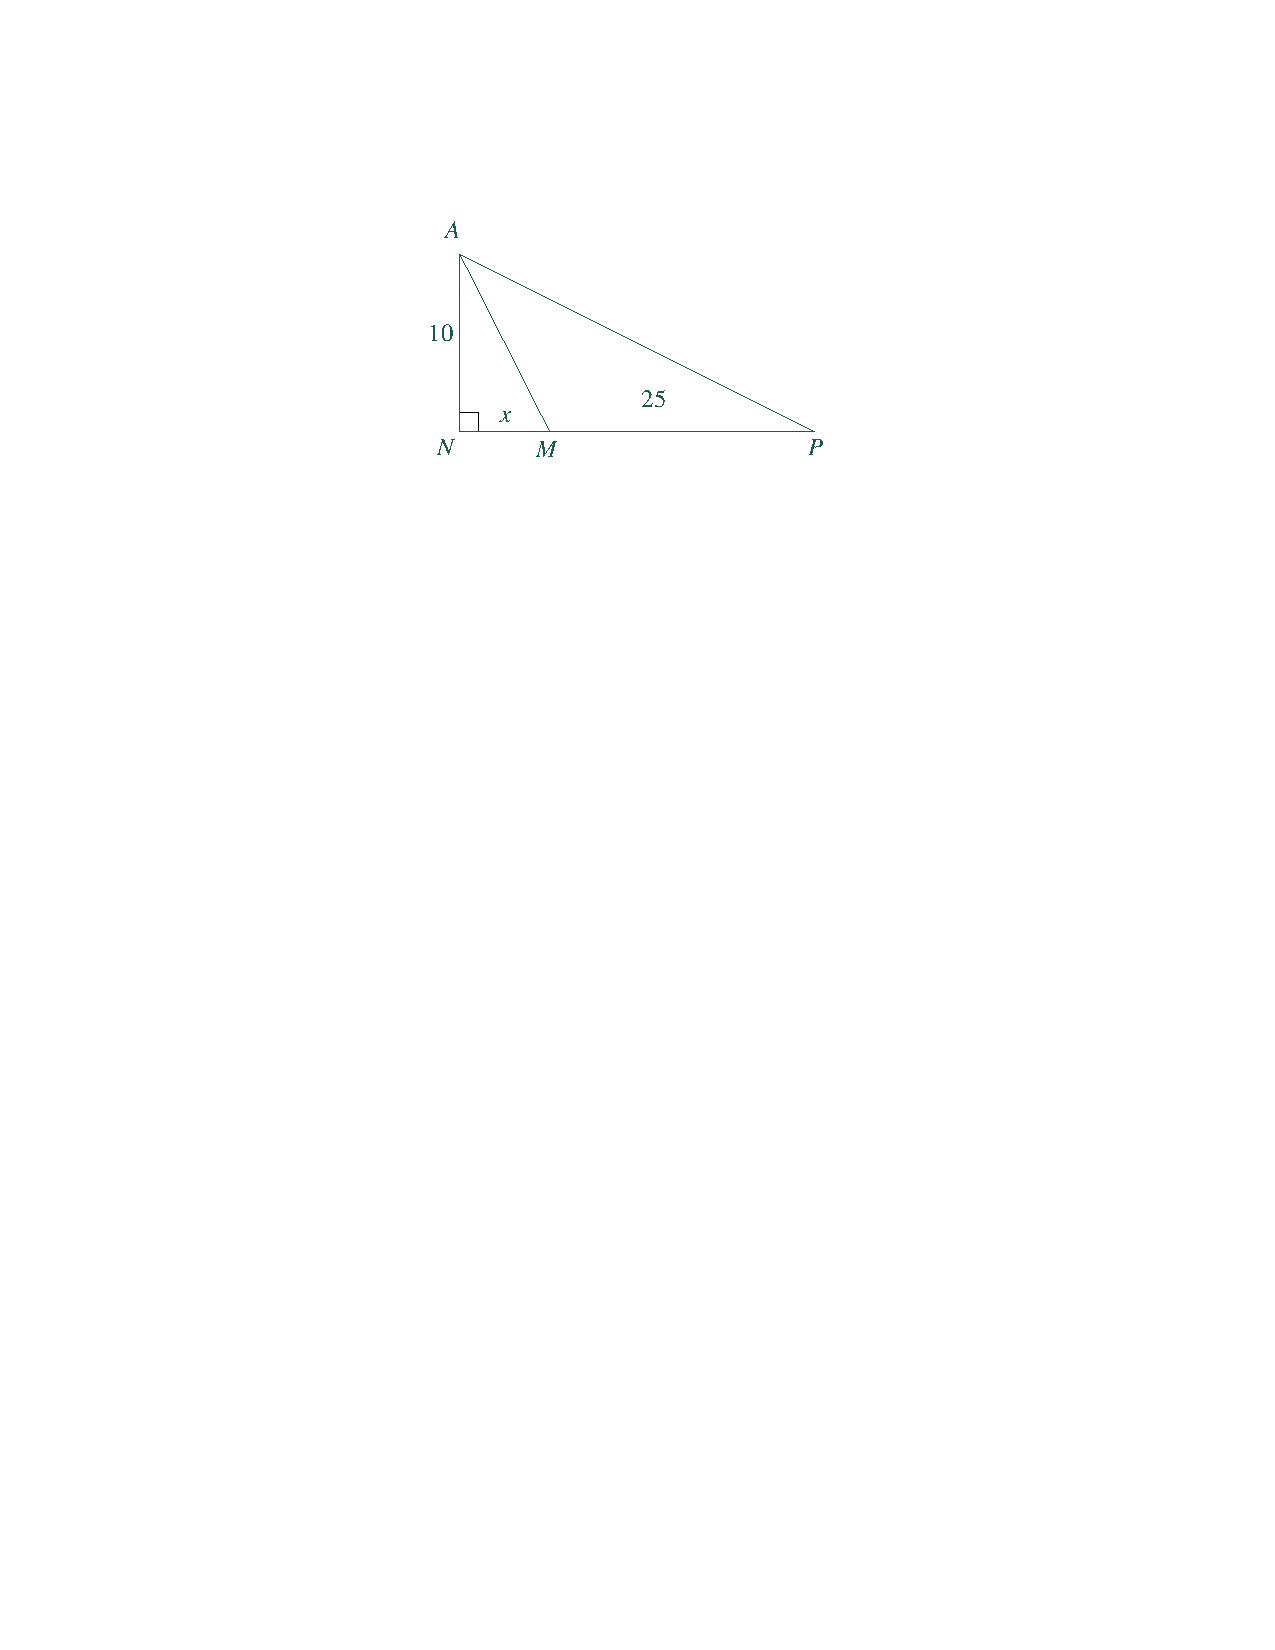
\includegraphics[width=.8\linewidth]{P597a}
		\vspace*{-10pt}
	\end{figure}
	$a)$ Vì $ANP$ là tam giác vuông tại $N$ nên ta có:
	\begin{align*}
		AP = \sqrt {A{N^2} + N{P^2}}  &= \sqrt {{{10}^2} + {{25}^2}}  \\
		&= 5\sqrt {29} \,({\text{\color{black}km}}).
	\end{align*}
	Do xe của nhà địa chất chỉ có thể chạy với vận tốc tối đa $30km/h$ trên sa mạc, nên để đi từ $A$ đến $P$ theo đường sa mạc, nhà địa chất cần đi trong ít nhất
	\begin{align*}
		\frac{{5\sqrt {29} }}{{30}} = \frac{{\sqrt {29} }}{6} \approx 0,898({\rm{h}}) \approx 54 \,(\text{\color{black}phút}).
	\end{align*}
	$b)$ Nếu nhà địa chất đi từ $A$ đến $N$, rồi đi theo con đường thẳng để đến $P$, thì thời gian đi tối thiểu là:
	\begin{align*}
		\frac{{10}}{{30}} + \frac{{25}}{{50}} = \frac{5}{6}({\rm{h}}) = 50 \,(\text{\color{black}phút}).
	\end{align*}
	Như vậy, nếu đi theo cách này thì nhà địa chất sẽ nhanh tới $P$ hơn, so với cách đi thẳng từ $A$ đến $P$ theo đường sa mạc.
	\vskip 0.05cm
	$c)$ Từ kết quả của câu $b)$ suy ra, cách đi nhanh nhất từ $A$ đến $P$ sẽ nằm trong số các cách đi sau: Đi thẳng theo đường sa mạc từ $A$ đến một địa điểm trên đoạn đường $NP$, rồi đi thẳng từ điểm đó đến $P$.
	\vskip 0.05cm
	Xét điểm $M$ tùy ý thuộc đoạn $NP$. Gọi $x$ (km) là độ dài quãng đường $NM$ (xem Hình vẽ ở cột bên trang trước). Khi đó, thời gian tối thiểu $t$ (tính theo đơn vị giờ) để đi thẳng từ $A$ đến $M$, theo đường sa mạc, rồi đi tiếp đến $P$, theo đường thẳng, sẽ là:
	\begin{align*}
		t = \frac{{\sqrt {{{10}^2} + {x^2}} }}{{30}} + \frac{{25 - x}}{{50}}.
	\end{align*}
	Ta cần xác định $x$ để $t$ nhận giá trị nhỏ nhất có thể.
	\vskip 0.05cm
	Theo bất đẳng thức Buniacopxki, ta có:
	\begin{align*}
			t &= \frac{{\sqrt {{{10}^2} + {x^2}} }}{{30}} + \frac{{25 - x}}{{50}} \\
			&= \frac{{\sqrt {{{10}^2} + {x^2}}  \cdot \sqrt {{{10}^2} + 7,{5^2}} }}{{30 \cdot \sqrt {{{10}^2} + 7,{5^2}} }} + \frac{{25 - x}}{{50}}\\
			 &\ge \frac{{10 \cdot 10 + 7,5x}}{{30 \cdot 12,5}} + \frac{{25 - x}}{{50}} = \frac{{23}}{{30}}.
	\end{align*}
	Dấu ``$=$" ở bất đẳng thức trên xảy ra khi và chỉ khi $x = 7,5$.
	\vskip 0.05cm
	Vì vậy, cách đi nhanh nhất từ $A$ đến $P$ là, đi thẳng theo đường sa mạc từ $A$ đến địa điểm $M$, nằm giữa $N$ và $P$, và cách $N$ $7,5$km, sau đó đi tiếp theo đường thẳng từ $M$ đến $P$. Đi theo cách này, thời gian đi tối thiểu sẽ là $\dfrac{23}{30}\text{h}$, hay $46$ phút.
	\vskip 0.05cm
	\textbf{\color{thachthuctoanhoc}Bình luận và Nhận xét}
	\vskip 0.05cm
	$\pmb{1.}$ Cách ``chính tắc", quen thuộc để tìm giá trị nhỏ nhất của $t$ ở câu $c)$ là: coi $t$ là hàm số của $x$, và khảo sát hàm số đó trên nửa khoảng $[0; 25)$. Có $60\%$ số bạn gửi lời giải tới Tạp chí đã giải câu $c)$ theo cách này (trong số đó có một bạn học sinh lớp $7$!).
	\vskip 0.05cm
	$\pmb{2.}$ Đánh giá giá trị của các biểu thức có chứa căn thức, bằng cách sử dụng bất đẳng thức Buniacopxki (còn gọi là bất đẳng thức Cauchy -- Schwarz), là một kỹ thuật đại số phổ dụng. Vì thế, nghĩ tới việc sử dụng bất đẳng thức vừa nêu để đánh giá giá trị của $t$ ở bài toán này là một cách tiếp cận tự nhiên. Điểm mấu chốt trong việc xử lý theo hướng này là tìm ra biểu thức thích hợp, cần mang nhân với biểu thức $\sqrt {{{10}^2} + {x^2}}$. Có thể thấy, nếu $t$ đạt giá trị nhỏ nhất tại $x = a$ thì dựa vào điều kiện xảy ra dấu bằng ở bất đẳng thức Buniacopxki, ta sẽ nghĩ đến biểu thức $\sqrt {{{10}^2} + {a^2}}$.  Thử nghiệm biểu thức này, ta thu được đánh giá:
	\begin{align*}
		t \ge \frac{{10 \cdot 10 + ax}}{{30 \cdot \sqrt {{{10}^2} + {a^2}} }} + \frac{{25 - x}}{{50}}.
	\end{align*}
	\textit{Câu hỏi đặt ra}: $a$ là số làm cho biểu thức ở vế phải của bất đẳng thức trên là biểu thức hằng, hay để tìm đến giá trị nhỏ nhất của $t$ còn cần các đánh giá tiếp theo? Nói một cách khác, liệu $a$ có phải là số sao cho
	\begin{align*}
		\frac{a}{{3 \cdot \sqrt {{{10}^2} + {a^2}} }} - \frac{1}{5} = 0?
	\end{align*}
	Lẽ dĩ nhiên, để trả lời được câu hỏi này, cần xem đẳng thức trên như một phương trình ẩn $a$, rồi giải phương trình ấy.
	\vskip 0.05cm
	Những điều vừa nêu trên chính là các suy diễn giúp tìm ra lời giải cho câu $c)$, đã trình bày ở trên.
	\vskip 0.05cm
	$\pmb{3.}$ Tất cả các lời giải Tạp chí nhận được từ bạn đọc đều là lời giải đúng.
	\begin{flushright}
		\textbf{\color{thachthuctoanhoc}Trần Nam Dũng}
	\end{flushright}
	{\color{thachthuctoanhoc}{\usefont{T5}{qag}{b}{n} P598.}}
	(Mức $A$) Chứng minh rằng,  tồn tại số tự nhiên có $2022$ chữ số, được tạo thành từ hai chữ số $4$, $5$ và chia hết cho $2^{2022}$.
	\vskip 0.05cm
	\textbf{\color{thachthuctoanhoc}Lời giải $\pmb{1}$} (\textit{dựa theo cách giải của bạn Hà Mạnh Hùng, lớp $7$A, trường THPT chuyên Hà Nội -- Amsterdam, Tp. Hà Nội})\textbf{\color{thachthuctoanhoc}.}
	\vskip 0.05cm
	Trước hết, ta có Nhận xét sau:
	\vskip 0.05cm
	\textbf{\color{thachthuctoanhoc}\textit{Nhận xét.}} Với $A = \overline {{a_{2021}}{a_{2020}} \ldots {a_1}{a_0}} $  là số tùy ý có $2022$ chữ số, ta có
	\begin{align*}
		A \equiv \overline {{a_{n - 1}} \ldots {a_0}} \left( {\bmod {2^n}} \right),
	\end{align*}
	với mọi $n \in \{1; 2; \ldots; 2021\}$.
	\vskip 0.05cm
	\textit{Chứng minh}. Với mọi $n \in \{1; 2; \ldots; 2021\}$, ta có:
	\begin{align*}
		A = \overline {{a_{2021}}{a_{2020}} \ldots {a_n}}  \cdot {10^n} + \overline {{a_{n - 1}} \ldots {a_0}} .
	\end{align*}
	Từ đó, do  ${10^n} \equiv 0\left( {\bmod {2^n}} \right)$, hiển nhiên suy ra khẳng định đã nêu ở Nhận xét.
	\vskip 0.05cm
	\textit{Trở lại bài toán}.
	\vskip 0.05cm
	Ký hiệu $S$ là tập hợp tất cả các số tự nhiên có $2022$ chữ số, có thể lập được từ hai chữ số $4$, $5$.
	\vskip 0.05cm
	Xét hai số $x = \overline {{x_{2021}}{x_{2020}} \ldots {x_1}{x_0}} $,\linebreak $y = \overline {{y_{2021}}{y_{2020}} \ldots {y_1}{y_0}} $  tùy ý thuộc $S$.
	\vskip 0.05cm
	Giả sử $x \equiv y\left( {\bmod {2^{2022}}} \right)$. \hfill ($1$)
	\vskip 0.05cm
	Khi đó, hiển nhiên có $x \equiv y\left( {\bmod 2} \right)$.  Vì thế, theo Nhận xét, ta có
	\begin{align*}
		{x_0} \equiv x \equiv y \equiv {y_0}\left( {\bmod 2} \right);
	\end{align*}
	mà ${x_0},{y_0} \in \left\{ {4;5} \right\}$ nên $x_0 = y_0$. \hfill ($2$)
	\vskip 0.05cm         
	Giả sử đã có  ${x_i} = {y_i}$ với mọi số tự nhiên $i$ mà $0 \le i \le k$, với $k$ là một số tự nhiên không vượt quá $2020$. Khi đó, do \linebreak$x \equiv y\left( {\bmod {2^{k + 2}}} \right)$  (suy ra từ ($1$)), và do
	\begin{align*}
		&\overline {{x_{k + 1}}{x_k} \ldots {x_0}}  = {x_{k + 1}} \cdot {10^{k + 1}} + \overline {{x_k} \ldots {x_0}} ,\\
		&\overline {{y_{k + 1}}{y_k} \ldots {y_0}}  = {y_{k + 1}} \cdot {10^{k + 1}} + \overline {{y_k} \ldots {y_0}} ,
	\end{align*}
	nên theo Nhận xét, ta có:
	\begin{align*}
		{x_{k + 1}} \cdot {10^{k + 1}} \equiv {y_{k + 1}} \cdot {10^{k + 1}}\left( {\bmod {2^{k + 2}}} \right).
	\end{align*}
	Suy ra
	\begin{align*}
		{x_{k + 1}} \cdot {2^{k + 1}} \equiv {y_{k + 1}} \cdot {2^{k + 1}}\left( {\bmod {2^{k + 2}}} \right);
	\end{align*}
	mà ${x_{k + 1}},{y_{k + 1}} \in \left\{ {4;5} \right\}$ nên  ${x_{k + 1}} = {y_{k + 1}}$.
	\vskip 0.05cm
	Vì thế, xuất phát từ ($2$), ta được $x_i = y_i$  với mọi $i \in \{0; 1; \ldots; 2021\}$. Do đó, $x = y$.
	\vskip 0.05cm
	Như vậy, với mọi $x, y \in S, x \ne y$, ta có  \linebreak$x\not  \equiv y\left( {\bmod {2^{2022}}} \right)$. Từ đây, do $S$ là tập gồm $2^{2022}$ số đôi một phân biệt nên $S$ là một hệ thặng dư đầy đủ modulo $2^{2022}$.  Vì thế, tồn tại số $a \in S$ sao cho $a \equiv 0\left( {\bmod {2^{2022}}} \right).$  Do 
	\begin{align*}
		&\underbrace {44 \ldots 4}_{2022{\text{ chữ số }}4}\not  \equiv 0\left( {\bmod {2^{2022}}} \right)\\
		\text{ \color{black} và } &\underbrace {55 \ldots 5}_{2022{\text{ chữ số }}5}\not  \equiv 0\left( {\bmod {2^{2022}}} \right),
	\end{align*}
	nên $a$ là số mà trong biểu diễn thập phân của nó có cả chữ số $4$ và chữ số $5$; vì thế, $a$ là số tự nhiên có $2022$ chữ số, được tạo thành từ hai chữ số $4, 5$.
	\vskip 0.05cm
	Ta có điều phải chứng minh theo yêu cầu đề bài.
	\vskip 0.05cm
	\textbf{\color{thachthuctoanhoc}Lời giải} $\pmb{2}$ (\textit{dựa theo cách giải của một bạn học sinh cấp THCS và hai bạn học sinh cấp THPT})\textbf{\color{thachthuctoanhoc}.}
	\vskip 0.05cm
	Trước hết, ta chứng minh Khẳng định sau:
	\vskip 0.05cm
	\textbf{\color{thachthuctoanhoc}\textit{Khẳng định.}} Với mỗi số nguyên dương $n$, ký hiệu $S_n$  là tập hợp tất cả các số có $n$ chữ số, có thể lập được từ hai chữ số $4$, $5$. Khi đó, với mọi số nguyên dương $n$, trong tập $S_n$   luôn có một số chia hết cho $2^n$.
	 \vskip 0.05cm
	\textit{Chứng minh}. Ta sẽ chứng minh Khẳng định bằng phương pháp quy nạp theo $n$.
	\vskip 0.05cm
	$\diamond$ Với $n = 1$, ta có ${S_1} = \left\{ {4;5} \right\}$.  Vì $4$ chia hết cho $2^1$  nên kết luận của Khẳng định là đúng, với $n = 1$.
	\vskip 0.05cm
	$\diamond$ Giả sử kết luận của Khẳng định là đúng, với $n = k$, $k \in \mathbb{N^*}$. Nghĩa là, trong tập $S_k$  tồn tại số $A$ chia hết cho $2^k$.
	\vskip 0.05cm 
	$\diamond$ Xét $n = k + 1$.
	\vskip 0.05cm
	Do $A \in S_k$  nên  $\overline {4A} ,\overline {5A}  \in {S_{k + 1}}$. \hfill ($1$)
	\vskip 0.05cm
	Nếu $A$ chia hết cho $2^{k+1}$  thì
	\begin{align*}
		\overline {4A}  &= 4 \cdot {10^k} + A = {2^{k + 2}} \cdot {5^k} + A \\
		&\equiv 0\left( {\bmod {2^{k + 1}}} \right). \tag{$2$}
	\end{align*}
	Nếu $A$ không chia hết cho $2^{k+1}$  thì  \linebreak$A \equiv {2^k}\left( {\bmod {2^{k + 1}}} \right)$; do đó
	\begin{align*}
		\overline {5A}  &= 5 \cdot {10^k} + A \\
		&= {2^k} \cdot \left( {{5^{k + 1}} + 1} \right) + \left( {A - {2^k}} \right)\\
		&\equiv 0\left( {\bmod {2^{k + 1}}} \right). \tag{$3$}
	\end{align*}
	Từ ($1$), ($2$) và ($3$) suy ra, trong $S_{k+1}$  tồn tại số chia hết cho $2^{k+1}$.
	\vskip 0.05cm 
	Như thế, kết luận của Khẳng định là đúng, với $n = k + 1$.
	\vskip 0.05cm
	$\diamond$ Theo nguyên lý quy nạp, Khẳng định được chứng minh.
	\vskip 0.05cm
	Áp dụng Khẳng định cho $n = 2022$, ta được: Trong $S_{2022}$ tồn tại số $X$ chia hết cho $2^{2022}$. Do
	\begin{align*}
		&\underbrace {44 \ldots 4}_{2022{\text{ chữ số }}4}\not  \equiv 0\left( {\bmod {2^{2022}}} \right)\\
		\text{\color{black} và } &\underbrace {55 \ldots 5}_{2022{\text{ chữ số }}5}\not  \equiv 0\left( {\bmod {2^{2022}}} \right),
	\end{align*}
	nên $X$ là số mà trong biểu diễn thập phân của nó có cả chữ số $4$ và chữ số $5$; vì thế, $X$ là số tự nhiên có $2022$ chữ số, được tạo thành từ hai chữ số $4$, $5$.
	\vskip 0.05cm
	Ta có điều phải chứng minh theo yêu cầu đề bài.
	\vskip 0.05cm
	\textbf{\color{thachthuctoanhoc}Bình luận và Nhận xét}
	\vskip 0.05cm
	$\pmb{1.}$ Rất tiếc, bạn học sinh cấp THCS và hai bạn học sinh cấp THPT, có ý giải như ở Lời giải $2$, có lời giải không đúng, do các bạn chưa chứng minh được số tự nhiên, thuộc $S_{2022}$ (theo ký hiệu trong Lời giải $2$) và chia hết cho $2^{2022}$ là số mà trong biểu diễn thập phân của nó có cả chữ số $4$ và chữ số $5$ (tức, là số được tạo thành từ hai chữ số $4$, $5$).
	\vskip 0.05cm
	\textbf{\color{thachthuctoanhoc}\textit{Lưu ý}} rằng, trong tiếng Việt, \textit{ta nói ``số $N$ \textbf{\color{thachthuctoanhoc}được tạo thành} từ các chữ số ..." khi và chỉ khi trong biểu diễn thập phân của $N$ có và chỉ có các chữ số ấy}. (Không ai nói, $1$ là số được tạo thành từ hai chữ số $1$, $2$ (chẳng hạn)!)
	\vskip 0.05cm
	$\pmb{2.}$ Lời giải của bạn \textit{Hà Mạnh Hùng} là lời giải đúng duy nhất, trong số các lời giải Tạp chí đã nhận được từ bạn đọc.
	\vskip 0.05cm
	$\pmb{3.}$ Dễ thấy, bằng phương pháp của Lời giải $1$, dễ dàng chứng minh được kết quả khái quát sau:
	\vskip 0.05cm
	\textbf{\color{thachthuctoanhoc}Kết quả khái quát.} \textit{Cho $a$ là một chữ số chẵn khác $0$, và $b$ là một chữ số lẻ. Khi đó, với mọi số nguyên dương $n$, trong số các số tự nhiên có $n$ chữ số, có thể lập được từ hai chữ số $a$, $b$, có đúng một số chia hết cho $2^n$.} 
	\vskip 0.05cm
	Kết quả khái quát nêu trên có Hệ quả hiển nhiên sau:
	\vskip 0.05cm
	\textbf{\color{thachthuctoanhoc}Hệ quả.} \textit{Cho $b$ là một chữ số lẻ. Khi đó:
	\vskip 0.05cm
	$1)$ Với mọi số nguyên dương $n \ge 2$, tồn tại duy nhất số tự nhiên có $n$ chữ số, \textbf{\color{thachthuctoanhoc}được tạo thành} từ hai chữ số $2$, $b$, và chia hết cho $2^n$.
	\vskip 0.05cm 
	$2)$ Với mọi số nguyên dương $n \ge 3$, tồn tại duy nhất số tự nhiên có $n$ chữ số, \textbf{\color{thachthuctoanhoc}được tạo thành} từ hai chữ số $4$, $b$, và chia hết cho $2^n$.
	\vskip 0.05cm 
	$3)$ Với mọi số nguyên dương $n \ge 2$, tồn tại duy nhất số tự nhiên có $n$ chữ số, \textbf{\color{thachthuctoanhoc}được tạo thành} từ hai chữ số $6$, $b$, và chia hết cho $2^n$.
	\vskip 0.05cm 
	$4)$ Với mọi số nguyên dương $n \ge 4$, tồn tại duy nhất số tự nhiên có $n$ chữ số, được tạo thành từ hai chữ số $8$, $b$, và chia hết cho $2^n$.}
	\vskip 0.05cm
		\hfill \textbf{\color{thachthuctoanhoc}Nguyễn Khắc Minh}
	\vskip 0.05cm
	{\color{thachthuctoanhoc}{\usefont{T5}{qag}{b}{n} P599.}}
	(Mức $A$) Cho các số thực dương $a$, $b$, $c$ có tổng bằng $7$. Chứng minh rằng
	\begin{align*}
		\frac{a}{b} + \frac{b}{c} + \frac{c}{a} + abc \ge ab + bc + ca - 2.
	\end{align*}
	\textbf{\color{thachthuctoanhoc}Lời giải} (\textit{theo Đáp án do Tạp chí cung cấp})\textbf{\color{thachthuctoanhoc}.}
	\vskip 0.05cm
	Với $f\left( {x,y,z} \right)$  là biểu thức của ba biến $x, y, z$, ký hiệu
	\begin{align*}
		\sum {f\!\left( {x,y,z} \right)}  \!=\! f\!\left( {x,y,z} \right) \!+\! f\!\left( {y,z,x} \right) \!+\! f\!\left( {z,x,y} \right)\!.
	\end{align*}
	Theo bất đẳng thức trung bình cộng -- trung bình nhân cho hai số thực không âm, ta có:
	\begin{align*}
		&\frac{a}{b} + \frac{{ab{{\left( {a - b + 2c} \right)}^2}}}{{49}} \ge \frac{2}{7}a\left( {a - b + 2c} \right).\\[-0.1ex]
		&\frac{b}{c} + \frac{{bc{{\left( {b - c + 2a} \right)}^2}}}{{49}} \ge \frac{2}{7}b\left( {b - c + 2a} \right).\\[-0.1ex]
		&\frac{c}{a} + \frac{{ca{{\left( {c - a + 2b} \right)}^2}}}{{49}} \ge \frac{2}{7}c\left( {c - a + 2b} \right).
	\end{align*}
	Cộng ba bất đẳng thức trên, vế theo vế, ta được:
	\begin{align*}
		&\frac{a}{b} + \frac{b}{c} + \frac{c}{a} + \sum {\frac{{ab{{\left( {a - b + 2c} \right)}^2}}}{{49}}}  \\[-0.1ex]
		\ge &\frac{2}{7}\sum {a\left( {a - b + 2c} \right)}. \tag{$1$}
	\end{align*}
	Tiếp theo, với lưu ý $a + b + c = 7$, ta có:
	\begin{align*}
			&\sum {ab{{\left( {a - b + 2c} \right)}^2}} \\[-0.1ex]
			 = &\sum ab\left( {a^2} + {b^2} + {c^2} - 2ab - 2bc - 2ca\right. \\[-0.1ex]
			 		&\left.+ 3{c^2} - 2bc + 6ca \right)\\[-0.1ex]
			 = &\left( {ab \!+\! bc \!+\! ca} \right)\!\!\left(\! {{a^2} \!+\! {b^2} \!+\! {c^2} \!-\! 2ab \!-\! 2bc \!-\! 2ca} \!\right) \\[-0.1ex]
			 &+\! abc\sum {\left( {6a \!-\! 2b \!+\! 3c} \right)} \\[-0.1ex]
			 = &\left( {ab \!+\! bc \!+\! ca} \right)\!\!{\left( {a \!+\! b \!+\! c} \right)^2} \!-\! 4{\left( {ab \!+\! bc \!+\! ca} \right)^2} \\[-0.1ex]
			 &+ 7abc\left( {a \!+\! b \!+\! c} \right)\\[-0.1ex]
			=&\,49\left( {ab \!+\! bc \!+\! ca} \right) \!-\! 4{\left( {ab \!+\! bc \!+\! ca} \right)^2} \\[-0.1ex]
			&\,+ 49abc. \tag{$2$}\\[-0.1ex]
		&\sum {a\left( {a - b + 2c} \right)}  \\[-0.1ex]
		= &\,{\left( {a + b + c} \right)^2} - \left( {ab + bc + ca} \right) \\[-0.1ex]
		= &\,\,49 - \left( {ab + bc + ca} \right). \tag{$3$}
	\end{align*}
	Thế ($2$) và ($3$) vào ($1$), ta được:
	\begin{align*}
		&\frac{a}{b} \!+\! \frac{b}{c} \!+\! \frac{c}{a} \!+\! \left( {ab \!+\! bc \!+\! ca} \right) \!-\! \frac{4}{{49}}{\left( {ab \!+\! bc \!+\! ca} \right)^2} \\
		&+\! abc \ge 14 \!-\! \frac{2}{7}\left( {ab \!+\! bc \!+\! ca} \right).
	\end{align*}
	Suy ra
	\begin{align*}
			&\frac{a}{b} + \frac{b}{c} + \frac{c}{a} + abc\\
			 \ge \,&\frac{4}{{49}}{\left( {ab \!\+\! bc \!+\! ca} \right)^2} \!-\! \frac{9}{7}\left( {ab \!+\! bc \!+\! ca} \right) \!+\! 14\\
			 = \,&\frac{4}{{49}}{\left( {ab \!+\! bc \!+\! ca \!-\! 14} \right)^2} \!+\! ab \!+\! bc \!+\! ca \!-\! 2\\
			 \ge \,&ab + bc + ca - 2.
	\end{align*}
	Bất đẳng thức của đề bài được chứng minh.
	\vskip 0.05cm
	\textbf{\color{thachthuctoanhoc}Bình luận và Nhận xét}
	\vskip 0.05cm
	$\pmb{1.}$ Với sự trợ giúp của phần mềm máy tính, có thể chứng minh được rằng, đẳng thức ở bất đẳng thức của đề bài xảy ra khi và chỉ khi $(a, b, c)$ là một hoán vị vòng quanh của  $\left( {4{{\sin }^2}\frac{{3\pi }}{7},4{{\sin }^2}\frac{{2\pi }}{7},4{{\sin }^2}\frac{\pi }{7}} \right)$.
	\vskip 0.05cm
	$\pmb{2.}$ Điểm mấu chốt ở lời giải trên là ``nhìn" ra ba bất đẳng thức dẫn đến bất đẳng thức ($1$) (trong lời giải đó). Đây là điều rất khó phát hiện.
	\vskip 0.05cm
	$\pmb{3.}$ Cách xử lý tự nhiên để chứng minh bất đẳng thức của đề bài là sử dụng phép đổi biến $q = ab + bc + ca$, $r = abc$. Tuy nhiên, bằng phương pháp này, bạn sẽ gặp phải các biến đổi hết sức cồng kềnh, phức tạp, rất khó thực hiện chỉ bằng ``giấy, bút". Bạn \textit{Trần Minh Hoàng} (lớp $9$E, trường THCS Nguyễn Trãi, huyện Nghi Xuân, tỉnh Hà Tĩnh) đã giải bài toán theo cách vừa nêu. Các biến đổi trong lời giải của bạn Hoàng quả thực rất phức tạp, các hệ số trong các biến đổi rất lớn, rất khó có thể tính được bằng tay. 
	\vskip 0.05cm
	$\pmb{4.}$ Lời giải của bạn \textit{Trần Minh Hoàng} là lời giải duy nhất Tạp chí nhận được từ bạn đọc; và là một lời giải đúng.
	\vskip 0.1cm
	\hfill	\textbf{\color{thachthuctoanhoc}Võ Quốc Bá Cẩn}
	\vskip 0.1cm
	{\color{thachthuctoanhoc}{\usefont{T5}{qag}{b}{n} P600.}}
	(Mức $A$) Cho $A$ là một tập con $100$ phần tử của tập hợp gồm $178$ số nguyên dương đầu tiên. Chứng minh rằng, với mỗi số $n$ thuộc tập hợp gồm $24$ số nguyên dương đầu tiên, đều tồn tại hai số thuộc $A$, có hiệu bằng $n$.
	\vskip 0.05cm
	\textbf{\color{thachthuctoanhoc}Lời giải} (\textit{phỏng theo ý giải của Đáp án do Tạp chí cung cấp})\textbf{\color{thachthuctoanhoc}.}
	\vskip 0.05cm
	Trong phần trình bày dưới đây, $|X|$  ký hiệu số phần tử của tập hữu hạn $X$.
	\vskip 0.05cm
	Ta sẽ giải bài đã ra bằng phương pháp phản chứng.
	\vskip 0.05cm
	Giả sử ngược lại, tồn tại số $n$ thuộc tập hợp gồm $24$ số nguyên dương đầu tiên, sao cho với mọi $x, y \in A$, $x \ne y$, đều có $|x - y| \ne n$.
	\vskip 0.05cm 
	Phân hoạch tập gồm $178$ số nguyên dương đầu tiên thành $n$ tập con  $S_1,  S_2, \ldots,  S_n$, sao cho hai số thuộc cùng một tập con khi và chỉ khi chúng đồng dư với nhau theo modulo $n$.
	\vskip 0.05cm
	Trong mỗi tập  $S_i$, $i = 1, 2, \ldots, n$, sắp xếp các số theo thứ tự tăng dần; khi đó, hai số thuộc $S_i$  có hiệu bằng $n$ khi và chỉ khi chúng là hai số liên tiếp trong sắp xếp đó. Vì thế, ở mỗi tập  $S_i$, $i = 1, 2, \ldots, n$, có không quá $\left\lceil {\frac{{\left| {{S_i}} \right| + 1}}{2}} \right\rceil$  số thuộc $A$. Do đó
	\begin{align*}
		100 = |A| \le \sum\limits_{i = 1}^n {\left\lceil {\frac{{\left| {{S_i}} \right| + 1}}{2}} \right\rceil}. \tag{$1$}
	\end{align*}
	Giả sử $178 = nq + r$, trong đó, $q$ là một số nguyên dương, và $r$ là một số tự nhiên, \linebreak$0 \le r \le n - 1$. Khi đó, trong phân hoạch nêu trên có $r$ tập con, mà mỗi tập con có $q + 1$ số, và $n - r$ tập con, mà mỗi tập con có $q$ số. Vì thế, theo ($1$), ta có:
	\begin{align*}
		100 \!\le\! r \!\cdot\! \left\lceil {\frac{{q \!+\! 2}}{2}} \right\rceil \!+\! \left( {n \!-\! r} \right) \!\cdot\!\left\lceil {\frac{{q \!+\! 1}}{2}}\right\rceil\!. \tag{$2$}
	\end{align*}
	Xảy ra hai trường hợp sau:
	\vskip 0.05cm
	$\diamond$ \textit{Trường hợp $1$. $q$ là số chẵn.}
	\vskip 0.05cm
	Khi đó, từ ($2$), ta có:
	\begin{align*}
		100 &\le r \cdot \frac{{q + 2}}{2} + \left( {n - r} \right) \cdot \frac{q}{2}\\
		 &= \frac{{nq}}{2} + r = \frac{{178 + r}}{2};
	\end{align*}
	suy ra, $r \ge 22$. Do đó, $n \ge r + 1 \ge 23$, và $nq = 178 - r \le 178 - 22 = 156$. Suy ra
	\begin{align*}
		q \le \frac{{156}}{n} \le \frac{{156}}{{23}} = 6\frac{{18}}{{23}};
	\end{align*}
	từ đó, do $q \in \mathbb{N^*}$  ta có $q \le 6$. Vì vậy
	\begin{align*}
		178 = nq + r \le 6n + r < 7n   \,\,(\text{\color{black}do }r < n);
	\end{align*}
	suy ra, $n > \dfrac{178}{7} > 25$,  mâu thuẫn với giả thiết $n \in \{1; 2; \ldots; 24\}$.
	\vskip 0.05cm
	$\diamond$ \textit{Trường hợp $2$. $q$ là số lẻ.}
	\vskip 0.05cm
	Khi đó, từ ($2$), ta có:
	\begin{align*}
		100 &\le r \cdot \frac{{q + 1}}{2} + \left( {n - r} \right) \cdot \frac{{q + 1}}{2} \\
		&= n \cdot \frac{{q + 1}}{2} = \frac{{178 + n - r}}{2}; \tag{$3$}
	\end{align*}
	suy ra, $n - r \ge 22$. Do đó, $n \ge 22 + r \ge 22$; vì vậy, $178 \ge nq \ge 22q$. Suy ra
	\begin{align*}
		q \le \frac{{178}}{{22}} = 8\frac{1}{{11}};
	\end{align*}
	từ đó, do $q$ là số nguyên dương lẻ nên $q \le 7$. Vì vậy, từ ($3$), ta có:
	\begin{align*}
		n \ge \frac{{200}}{{q + 1}} \ge \frac{{200}}{8} = 25,
	\end{align*}
	mâu thuẫn với giả thiết $n \in \{1; 2; \ldots; 24\}$.
	\vskip 0.05cm
	Các mâu thuẫn nhận được từ việc xét hai trường hợp trên cho thấy, giả sử phản chứng là sai. Vì thế, ta có điều phải chứng minh theo yêu cầu đề bài.
	\vskip 0.05cm
	\textbf{\color{thachthuctoanhoc}Bình luận và Nhận xét}
	\vskip 0.05cm
	$\pmb{1.}$ Theo tác giả bài toán, với $n$ là số nguyên dương lớn hơn $24$, sẽ tồn tại tập con $A$ có $100$ phần tử của tập hợp $178$ số nguyên dương đầu tiên, sao cho với mọi $x, y \in A$, $x \ne y$, đều có $|x-y| \ne n$.
	\vskip 0.05cm 
	$\pmb{2.}$ Theo đánh giá của người chấm bài, bài đã ra là một bài toán nhẹ nhàng (vì có dạng quen thuộc), và thú vị. Tiếc rằng, cho đến thời điểm bản thảo vào Nhà in, Tạp chí vẫn chưa nhận được một lời giải nào từ bạn đọc.
	\vskip 0.15cm
	\hfill	\textbf{\color{thachthuctoanhoc}Nguyễn Khắc Minh}
	\vskip 0.15cm
	\rule{1\linewidth}{0.1pt}
	\vskip 0.1cm
	\textbf{\color{thachthuctoanhoc}ĐÍNH CHÍNH}
	\vskip 0.1cm
	\textit{Các dòng từ $1$ đến $7$ (trên xuống), cột bên trái, trang $33$, Tạp chí Pi Tập $6$, số tháng $6/2022$, được sửa lại như sau:}
	\vskip 0.05cm
	``Từ ($2$) và ($3$), suy ra $e \ge 5$. Vì thế, từ ($1$), với lưu ý $a$, $b$, $c$, $d$ là các số nguyên, ta được: $d \ge 6$, $c \ge 7$, $b \ge 8$ và $a \ge 9$. Do đó
	\begin{align*}
		S \ge &\,9 \cdot 8 \cdot 7 \cdot 6 + 9 \cdot 8 \cdot 7 \cdot 5 + 9 \cdot 8 \cdot 6 \cdot 5 \\
		&+ 9 \cdot 7 \cdot 6 \cdot 5 + 8 \cdot 7 \cdot 6 \cdot 5 = 11274.
	\end{align*}
	Dấu bằng đạt được khi $a = 9$, $b = 8$, $c = 7$, $d = 6$ và $e = 5$."
	\vskip 0.05cm
	\textit{Thành thật cáo lỗi cùng bạn đọc.}
\end{multicols}
\begin{center}
	\textbf{\color{thachthuctoanhoc}DANH SÁCH HỌC SINH CÓ LỜI GIẢI HOÀN CHỈNH}
\end{center}
\begin{multicols}{2}
	\textit{Trong các ngoặc đơn ở phần dưới đây, sau tên lớp là mã hiệu của các bài toán mà học sinh có lời giải hoàn chỉnh.}
	\vskip 0.05cm
	\textbf{\color{thachthuctoanhoc}KHỐI THCS}
	\vskip 0.05cm
	$\bullet$ Trường \textbf{\color{thachthuctoanhoc}THCS Sơn Đồng}, huyện Hoài Đức, Tp. Hà Nội: \textit{Nguyễn Đăng Dũng} (lớp $9$A$1$; P$593$, P$595$).
	\vskip 0.05cm
	$\bullet$ Trường \textbf{\color{thachthuctoanhoc}THPT chuyên Hà Nội -- Amsterđam}, Tp. Hà Nội: \textit{Hà Mạnh Hùng} (lớp $7$A; P$591$, P$592$, P$593$, P$597$, P$598$).
	\vskip 0.05cm
	$\bullet$ Trường \textbf{\color{thachthuctoanhoc}THCS Nguyễn Trãi}, huyện Nghi Xuân, tỉnh Hà Tĩnh: \textit{Trần Minh Hoàng} (lớp $9$E; P$591$, P$592$, P$593$, P$594$, P$595$, P$596$, P$597$, P$599$).
	\vskip 0.05cm
	$\bullet$ Trường \textbf{\color{thachthuctoanhoc}THCS Nguyễn Trãi}, huyện Đại Lộc, tỉnh Quảng Nam: \textit{Nguyễn Châu Tuấn Kiệt} (lớp $9/7$; P$593$, P$595$, P$596$).
	\vskip 0.05cm
	$\bullet$ Trường \textbf{\color{thachthuctoanhoc}THCS Chu Văn An}, tỉnh Thừa Thiên -- Huế: \textit{Phan Đặng Hữu Toàn} (lớp $9$A; P$595$).
	\vskip 0.05cm
	\textbf{\color{thachthuctoanhoc}KHỐI THPT}
	\vskip 0.05cm
	$\bullet$ Trường \textbf{\color{thachthuctoanhoc}THPT số $\pmb{2}$ Phù Cát}, tỉnh Bình Định: \textit{Nguyễn Hữu Trí} (lớp $10$A$1$; P$594$, P$595$, P$596$).
	\vskip 0.05cm
	$\bullet$ Trường \textbf{\color{thachthuctoanhoc}THPT chuyên Nguyễn Quang Diêu}, tỉnh Đồng Tháp: \textit{Nguyễn Chí Việt Khang} (lớp $11$T$1$; P$593$, P$594$, P$595$), \textit{Đỗ Duy Quang} (lớp $10$T$1$; P$595$), \textit{Lâm Nhật Tiến} (lớp $10$T$1$; P$595$).
	\vskip 0.05cm
	$\bullet$ Trường \textbf{\color{thachthuctoanhoc}THPT Gia Định}, Tp. Hồ Chí Minh: \textit{Lê Anh Khoa} (lớp $10$CT; P$594$), \textit{Nguyễn Hà Ngọc Uyên} (lớp $11$CT; P$595$).
	\vskip 0.05cm
	$\bullet$ Trường \textbf{\color{thachthuctoanhoc}THPT chuyên Hưng Yên}, tỉnh Hưng Yên: \textit{Trần Hữu Dương} (lớp $10$ Toán $1$; P$596$), \textit{Vũ Quang Hòa} (lớp $10$ Toán $1$; P$593$), \textit{Nguyễn Gia Khánh} (lớp $10$ Toán $1$; P$597$).
	\vskip 0.05cm
	$\bullet$ Trường \textbf{\color{thachthuctoanhoc}THPT chuyên Thăng Long}, tỉnh Lâm Đồng: \textit{Lương Nguyễn Gia Bảo} (lớp $10$ Toán; P$592$, P$594$, P$596$), \textit{Đặng Nguyễn Trường Giang} (lớp $10$ Toán; P$596$), \textit{Nguyễn Anh Khoa} (lớp $10$ Toán; P$592$, P$594$, P$595$, P$596$, P$597$).
	\vskip 0.05cm
	$\bullet$ Trường \textbf{\color{thachthuctoanhoc}THPT chuyên Lê Hồng Phong}, tỉnh Nam Định: \textit{Nguyễn Đức Khải} (lớp $10$ Toán $2$; P$593$, P$594$, P$595$, P$596$), \textit{Ninh Thị Mai Linh} (lớp $11$ Toán $1$; P$594$), \textit{Trần Đình Nam} (lớp $10$ Toán $2$; P$592$, P$593$, P$594$).
	\vskip 0.05cm
	$\bullet$ Trường \textbf{\color{thachthuctoanhoc}THPT chuyên Hùng Vương}, tỉnh Phú Thọ: \textit{Vũ Công Tâm} (lớp $10$ Toán; P$595$).
	\vskip 0.05cm
	$\bullet$ Trường \textbf{\color{thachthuctoanhoc}THPT chuyên Quốc học Huế}, tỉnh Thừa Thiên -- Huế: \textit{Võ Khắc Minh Hoàng} (lớp $10$ Toán $2$; P$596$, P$597$), \textit{Trần Thị Thanh Thư} (lớp $11$ Toán $1$; P$592$, P$593$, P$594$).
	\vskip 0.05cm
	$\bullet$ Trường \textbf{\color{thachthuctoanhoc}THPT chuyên Khoa học tự nhiên}, ĐH Khoa học tự nhiên -- ĐHQG Hà Nội: \textit{Nguyễn Cung Thành} (lớp $10$A$1$ Toán; P$595$, P$596$).
	\vskip 0.05cm
	$\bullet$ Trường \textbf{\color{thachthuctoanhoc}THPT chuyên Sư phạm}, ĐH Sư phạm Hà Nội: \textit{Hồ Trần Khánh Linh} (lớp $11$ Toán $2$; P$595$).
\end{multicols}
\vspace*{-10pt}
\rule{1\linewidth}{0.1pt}
\begin{center}
	\textbf{\Large\color{thachthuctoanhoc}LỜI GIẢI, ĐÁP ÁN}
\end{center}
\begin{multicols}{2}
	\textbf{\color{thachthuctoanhoc}Đố vui}
	\vskip 0.1cm 
	Có thể dễ dàng chỉ ra rằng với hai chiếc máy bay, Pi không thể thực hiện được kế hoạch của mình. Với ba chiếc máy bay thì Pi có thể thực hiện được, chẳng hạn với chiến lược sau~đây.   
	\vskip 0.1cm
	Đầu tiên, ba máy bay, một chiếc của Pi và hai chiếc khác để hỗ trợ Pi, cùng xuất phát từ sân bay. Sau khi đi được $1/8$ vòng Trái Đất, một máy bay tiếp nhiên liệu cho cả máy bay của Pi và chiếc còn lại, mỗi chiếc $1/4$ bình (nếu coi mỗi chiếc máy bay có $1$ bình nhiên liệu) và giữ lại cho mình $1/4$ bình. Khi này, hai chiếc máy bay có đầy bình và một chiếc có $1/2$ bình (vừa đủ để có thể quay lại sân bay ban đầu). Sau đó, hai máy bay có đầy bình tiếp tục hành trình của mình còn chiếc còn $1/2$ bình quay trở lại sân bay ban đầu. 
	\vskip 0.1cm
	Sau khi tiếp tục đi được $1/8$ vòng Trái Đất, nghĩa là được $1/4$ vòng kể từ điểm xuất phát, chiếc còn lại chuyển $1/4$ bình nhiên liệu cho Pi. Khi này Pi có đầy bình và chiếc còn lại có $1/4$ bình, vừa đủ để quay trở lại. Bây giờ, Pi tiếp tục hành trình của mình còn chiếc máy bay kia quay trở lại sân bay ban đầu. Với đầy bình, Pi có thể đi được $3/4$ vòng Trái Đất kể từ điểm xuất phát. 
	\vskip 0.1cm
	Máy bay đầu tiên, với đầy bình bay theo hướng ngược lại (so với hướng ban đầu) để 
	khi đó máy bay đầu tiên còn $1/2$ bình sẽ tiếp cho máy bay của Pi $1/4$ bình, sao cho cả hai máy bay có $1/4$ bình, đủ để đi đến vị trí $7/8$ vòng Trái Đất. Khi hai chiếc máy bay này gặp nhau, chiếc còn lại bắt đầu xuất phát từ sân bay ban đầu với đầy bình và bay theo hướng ngược lại để gặp máy bay của Pi và chiếc thứ hai ở vị trí $7/8$ vòng Trái Đất và tiếp cho mỗi chiếc $1/4$ bình. Khi này, mỗi chiếc có đúng $1/4$ bình, vừa đủ để bay về sân bay ban đầu.   
	\vskip 0.1cm
	\hfill (\textit{Xem tiếp trang} $62$.)
\end{multicols}
